% LaTeX-Vorlage Version 3.0,  Juni 2010
% erstellt von Dr. Andreas Drauschke und Dr. Susanne Teschl
% Modifiziert von Dr. Andreas Mehrle (andreas.mehrle@mci.edu)

%MODIFIZIERT von M. Panny - Version 1.8.0

\documentclass[a4paper, oneside, 10pt]{article}

\newcounter{RoemischeSeiten}
\pagenumbering{Roman}

\usepackage[dvips]{graphicx}
\usepackage[tmargin=1in,bmargin=1in,lmargin=1.25in,rmargin=1.25in]{geometry}
\usepackage{titlesec}
\usepackage{xcolor}
\usepackage[overload]{textcase}
\usepackage[utf8]{inputenc}
\usepackage{epstopdf}
\usepackage{listings}
\usepackage{wallpaper}
\usepackage[binary-units=true]{siunitx} %Zusätzliche Option erlaubt binary-units wie z.B.: \byte
\usepackage{placeins} %Für \FloatBarrier beim Einfügen von Abbildungen
%=============================================
\usepackage{exscale,relsize}
\usepackage{fancyhdr}
\usepackage[small]{caption}
\usepackage{float}
\usepackage{amsmath, amssymb, amsfonts, amsthm}
\usepackage{pst-all}
\usepackage{rotating}
\usepackage{mathrsfs}
\usepackage{makeidx}
\usepackage{multirow}
%=============================================
\usepackage{pgfplots}
\usepackage{tikz}
%\usepackage[european, siunitx]{circuitikz}
%=============================================
\usepackage{setspace} 
\usepackage{booktabs}
\usepackage{graphicx}
\usepackage{cancel}
\usepackage{xspace}
%=============================================
\usepackage{subcaption}
\usepackage{pdfpages}
\usepackage{nameref}
\usepackage[pdftex,bookmarks=true,bookmarksnumbered=true]{hyperref}
\usepackage{wasysym}
%=============================================
%STEINMETZ
%\PassOptionsToPackage{original}{pict2e} falls Probleme zw. cancel und steinmetz auftreten
\usepackage{steinmetz}	%für Versor/Phasor Symbol für Winkel in der Elektrotechnik 
%=============================================

%FONTS für \ttfamily und \bfseries gleichzeitig --> wird normal nicht unterstützt
%http://www.macfreek.nl/memory/LaTeX_Bold_Typewriter_Font
\DeclareFontShape{OT1}{cmtt}{bx}{n}{<5><6><7><8><9><10><10.95><12><14.4><17.28><20.74><24.88>cmttb10}{}

%SPRACHEN einrichten --> für Englisch: [main=english, ngerman] --> es muss evtl. 2x kompiliert werden
\usepackage[english]{babel}

\def\headerLists{headerLists}
\iflanguage{ngerman}{\def\headerLists{Verzeichnisse}}{}
\iflanguage{ngerman}{\def\headerLists{Indices}}{}
\iflanguage{ngerman}{\renewcommand\lstlistlistingname{Quellcodeverzeichnis}}{}
\iflanguage{ngerman}{\renewcommand\lstlistlistingname{List of \lstlistingname s}}{}
\expandafter\addto\csname captionsngerman\endcsname{\renewcommand{\refname}{Literaturverzeichnis}}

%Einstellung für TOC, damit lange Seitennummer (römisch) nicht zu weit rechts steht --> Wert muss angepasst werden
\makeatletter
\renewcommand{\@pnumwidth}{1.55em}	%default = 1.55em
\makeatother

%===================================================================

%FARBEN für Deckblatt, etc.
\def\isBlackAndWhite{1}
\if\isBlackAndWhite1
	\definecolor{MSBlue}{rgb}{0, 0, 0}
	\definecolor{MSLightBlue}{rgb}{0, 0, 0}
	%für listings
	\definecolor{lstGreen}{RGB}{0, 0, 0}
	\definecolor{lstBlue}{RGB}{0, 0, 0}
	\definecolor{lstGreenMatlab}{RGB}{0, 0, 0}
	\definecolor{lstLila}{RGB}{0, 0, 0}
\else
	\definecolor{MSBlue}{rgb}{0.204, 0.353, 0.541}
	\definecolor{MSLightBlue}{rgb}{0.31, 0.506, 0.741}
	%für listings
	\definecolor{lstGreen}{RGB}{46, 109, 103}
	\definecolor{lstBlue}{RGB}{40, 38, 160}
	\definecolor{lstGreenMatlab}{RGB}{28,172,0}
	\definecolor{lstLila}{RGB}{170,55,241}
\fi

%===================================================================

%FORMATS for each heading level
%\titleformat*{\section}{\rmfamily\bfseries\huge\color{MSBlue}\lowercase}
\setcounter{secnumdepth}{4}
\titleformat{\section}[hang]{\sffamily\bfseries\huge\color{MSBlue}}{\thesection}{1em}{}[]
\titleformat{\subsection}{\large\bfseries\sffamily\uppercase}{\thesubsection}{1em}{}
\titleformat{\subsubsection}{\sffamily\bfseries}{\thesubsubsection}{1em}{}
\titleformat{\paragraph}{\sffamily\bfseries}{\theparagraph}{1em}{}
\newcommand{\subsubsubsection}{\paragraph}
\titleformat{\subparagraph}{\sffamily\bfseries}{\thesubparagraph}{1em}{}
\newcommand{\subsubsubsubsection}{\subparagraph}

%\newcommand{\subsubsubsection}{\textbf}
%===================================================================

%SIUNITX
\iflanguage{ngerman}{\sisetup{locale=DE, tophrase={~bis~}}}{}		%Macht z.B.: Komma zum Dezimalseparator
\DeclareSIUnit{\var}{var}	%Volt-Ampere-Reaktiv
\DeclareSIUnit{\VA}{VA}		%Volt-Ampere
\DeclareSIUnit{\Nm}{\newton \meter}		%Newtonmeter
\DeclareSIUnit{\mm}{\milli \meter}		%Millimeter
\DeclareSIUnit{\Npsmm}{\newton \per \square \milli \meter}	%Newton-pro-Quadratmillimeter
\DeclareSIUnit{\decade}{dec}
%===================================================================

%LISTINGS for inline source code highlighting
\lstdefinelanguage{ST}{	%settings für Strukturierten Text
	keywords = {
		PROGRAM, CONFIGURATION, END_CONFIGURATION, VAR, VAR_GLOBAL, VAR_EXTERNAL, END_VAR, TASK, INTERVAL, AT, EXIT, WITH, VAR_INPUT, VAR_OUTPUT,
		IF, ELSE, ELSIF, THEN, END_IF, CASE, OF, END_CASE, RETURN,
		REPEAT, UNTIL, END_REPEAT, WHILE, END_WHILE, FOR, END_FOR, DO, TO, BY,
		BOOL, BYTE, WORD, DWORD, LWORD,
		INT, SINT, DINT, LINT, USINT, UINT, LDINT, ULINT, 
		REAL, LREAL, 
		ADR, TRUNC, ABS, SQRT, LN, LOG, EXP, SIN, COS, TAN, ASIN, ACOS, ATAN, EXPT,
		STRING, TIME, DATE, TIME_OF_DAY, DATE_AND_TIME,
		NOT, AND, OR, XOR, TRUE, FALSE, MOD, EXPT, FUNCTION_BLOCK
	},
	sensitive = true,			%case sensitivity --> should probably be false
	morecomment = [l]{//},		%inline comment
	morecomment = [s]{(*}{*)},	%mult line comment
	morecomment = [s]{/*}{*/},
	morestring = [b]",
	morestring = [b]',
	tabsize = 4
}

%default style for ST --> language must not be specified when using style
\lstdefinestyle{ST}{
	language=ST,
	basicstyle=\small\ttfamily,
	keywordstyle=\color{lstBlue}\bfseries,
	columns=fullflexible,
	breaklines=true,
	postbreak=\mbox{$\hookrightarrow$\space},
	captionpos=t,	%t for top or b for bottom
	commentstyle=\color{lstGreen}\itshape,
}

%default style for MATLAB --> language must not be specified when using style
\lstdefinestyle{matlab}{
	language=Matlab,
	basicstyle=\small\ttfamily,
	keywordstyle=[1]\color{lstBlue}\bfseries,
	keywordstyle=[2]\color{lstLila},
	commentstyle=\color{lstGreenMatlab}\itshape,
	stringstyle=\color{lstLila},
	showstringspaces=false,
	captionpos=t,
	tabsize = 4,
	columns=fullflexible,
	breaklines=true,
	postbreak=\mbox{$\hookrightarrow$\space},
	morekeywords={xlim,ylim,var,alpha,factorial,poissrnd,normpdf,normcdf,clearvars},
	%Put MATLAB function parameters here
	morekeywords=[2]{step_PT1, step_PT1T, step_PT2},
	morecomment=[l][\color{blue}]{...},     % Line continuation (...) like blue comment
}

%===================================================================

%TIKZ
\newcommand{\tikzDrawBB}{\draw (current bounding box.north east) -- (current bounding box.north west) -- (current bounding box.south west) -- (current bounding box.south east) -- cycle;}

%===================================================================
\numberwithin{figure}{section}
\numberwithin{table}{section}

% auxillary symbols
\renewcommand{\tilde}{\symbol{126}}
\newcommand{\define}{\stackrel{!}{=}}
\renewcommand{\equiv}{\,\widehat{=}\,}

\newcommand{\im}{j}
\newcommand{\matlab}{MATLAB\xspace}
\newcommand{\labview}{LabVIEW\xspace}
\newcommand{\simulink}{Simulink\xspace}
\newcommand{\flexsim}{FlexSim\xspace}

% format specifications
\newcommand{\ten}[1]{\mathbf{#1}}	%Tensor
\newcommand{\mat}[1]{\mathbf{#1}}	%Matrix

% mathematical operators
\newcommand{\grad}{\,\mathrm{grad}\,}
\renewcommand{\div}{\,\mathrm{div}\,}
\newcommand{\rot}{\,\mathrm{rot}\,}
\newcommand{\lap}{\Delta}
\newcommand{\laplace}[1]{\mathscr{L}\left\{#1\right\}}	%Laplacetransformation
\newcommand{\invLaplace}[1]{\mathscr{L}^{-1}\left\{#1\right\}}	%inverse Laplactransformation
\newcommand{\trans}{^{\raisebox{\depth - 0.075em}{$\intercal$}}}%{^T}	%Transponiert --> für Matrix
\DeclareMathSymbol{*}{\mathbin}{symbols}{"01} % Punkt statt *

%===================================================================

%Grad als Einheit --> °
\newcommand{\gradU}[1]{\SI{#1}{\degree}} %hauptsächlich in kombination mit steinmetz-package sinnvoll

%Toleranzen
\newcommand{\tol}[4]{\ensuremath{\SI{#1}{#2}^{+\num{#3}}_{-\num{#4}}}}	%#1 #2 +#3 -#4
\newcommand{\tolSingle}[3]{\ensuremath{\SI{#1}{#2}^{+\num{#3}}}}

%command für römische Zahlen
\newcommand{\RN}[1]{\textup{\uppercase\expandafter{\romannumeral#1}}}

%circled numbers (normal, big and small)
\newcommand{\circText}[1]{{\large \textcircled{\small{#1}}}}
\newcommand{\circTextBig}[1]{{\Large \textcircled{\normalsize{#1}}}}
\newcommand{\circTextSmall}[1]{{\textcircled{\small{#1}}}}

%command für dx, etc. für Integral
\newcommand{\diff}{\mathop{}\!\mathrm{d}}	%\diff x --> dx
\newcommand{\Diff}[1]{\mathop{}\!\mathrm{d^{#1}}} %\Diff[2] x --> d²x

%command für Ableitungen (normal und partiell) --> Verwendung austauschbar:
%\deriv{I}{t} --> dI/dt
%\deriv[2]{s}{t} --> d^2 s/dt^2
\newcommand{\deriv}[3][]{\frac{\Diff{#1} #2}{\diff {#3}^{#1}}}
\newcommand{\parDeriv}[3][]{\frac{\partial^{#1} #2}{\partial {#3}^{#1}}}

%command für nicht kursives e im Mathmode --> soll nicht kursiv sein, da eine Konstante
\newcommand{\eUpr}{\mathrm{e}}

%===================================================================
%ENVIRONMENTS

%small matrix mit eckigen Klammern
\newenvironment{bsmallmatrix}{\left[\begin{smallmatrix}}{\end{smallmatrix}\right]}

%===================================================================

\setlength{\parindent}{0em}
\setlength{\parskip}{1.5ex plus0.5ex minus0.5ex}
\setlength{\captionmargin}{3em}

\newcommand{\textdirectcurrent}{%
	\settowidth{\dimen0}{$=$}%
	\vbox to .85ex {\offinterlineskip
		\hbox to \dimen0{\leaders\hrule\hfill}
		\vskip.35ex
		\hbox to \dimen0{%
			\leaders\hrule\hskip.2\dimen0\hfill
			\leaders\hrule\hskip.2\dimen0\hfill
			\leaders\hrule\hskip.2\dimen0
		}
		\vfill
	}%
}
\newcommand{\mathdirectcurrent}{\mathrel{\textdirectcurrent}}







%============================= MATLAB STYLE ======================================
\lstdefinestyle{MStyle}{
    backgroundcolor=\color{backgroundColour},   
    language=Matlab, 
%    frame=single,
    basicstyle=\small\ttfamily,
    keywordstyle=[1]\color{Blue}\bfseries,  % MATLAB functions
    keywordstyle=[2]\color{Purple},         % MATLAB function arguments
    keywordstyle=[3]\color{Blue}\underbar,  % User functions
    identifierstyle=,                       % Nothing special about identifiers
    commentstyle=\usefont{T1}{pcr}{m}{sl}\color{MyDarkGreen}\small,
    stringstyle=\color{Purple},
    %%% Put standard MATLAB functions not included in the default
   %%% language here
    morekeywords={xlim,ylim,var,alpha,factorial,poissrnd,normpdf,normcdf},
    %%% Put MATLAB function parameters here
    morekeywords=[2]{on, off, interp},
    %%% Put user defined functions here
    morekeywords=[3]{FindESS, homework_example},
    morecomment=[l][\color{Blue}]{...},     % Line continuation (...) like blue comment
    numbers=left,
    firstnumber=1,
    numberstyle=\tiny\color{mGray},
    numbersep=5pt,
    stepnumber=5,
    showspaces=false,                
    showstringspaces=false,
    showtabs=false,                  
    tabsize=2,
}

\usepackage{xcolor}
\definecolor{Purple}{rgb}{0.71,0,1}
\definecolor{Black}{rgb}{0,0,0}
\definecolor{Blue}{rgb}{0,0,1}
\definecolor{mGreen}{rgb}{0,0.6,0}
\definecolor{mGray}{rgb}{0.5,0.5,0.5}
\definecolor{mPurple}{rgb}{0.58,0,0.82}
\definecolor{backgroundColour}{rgb}{0.95,0.95,0.92}
\definecolor{MyDarkGreen}{rgb}{0,0.8,0}
%============================= MATLAB STYLE ======================================


% LABORTITEL
\def\thesis{Report}
\def\labtitle{Laboratory Advanced Control Engineering}
\def\labcode{BB MECH-M-1-RTV-RTV-LB}
\def\labdate{13.01.2024 and 02.02.2024}

% LABORNAME & NUMMER
\def\labname{Lab 1 - Aerodynamic Levitation}
%\def\labnum{2}

% ANGABEN ZUM Studium & Student
\def\study{Master Mechatronics \& Smart Technologies}
\def\term{1.}
\def\lecturer{Jasper Volmer}
\def\group{MA-MECH-23-BB-2B}
\def\student{Lukas Figl, Lukas Sieß, Stefan Widmann}

\begin{document}

%\layout
\setlength{\belowcaptionskip}{-8pt}
 %Abstand nach Abbildungen von 0.0pt auf -8pt verringern

% Kopf- und Fusszeilen initiieren
\pagestyle{plain}

\thispagestyle{empty}
\sffamily

\ThisTileWallPaper{\paperwidth}{\paperheight}{Images/MCIHintergrundKPL.pdf}
%\put(-30,-685){\includegraphics[width=1.15\linewidth]{BG}}

{
	\bfseries

	\vspace*{3.5cm}

	\textcolor{MSBlue}{\sffamily\bfseries\huge\thesis}%

	\vspace*{0.5cm}

	\begin{doublespace} 
		
\textbf{\labtitle{} (\labcode)}

\textbf{\labname}

\textbf{\labdate}	

%Labor \labnum

	%\maketitle
	\vspace*{10cm}

	\textcolor{gray}{\study}

	\def\termname{Semester}
	\textcolor{gray}{\term{ }\termname}

	\def\lecturername{Lector}
	\textcolor{gray}{\lecturername: \lecturer}

	\def\groupname{Group}
	\textcolor{gray}{\groupname: \group}

	\def\authorname{Authors}
	\textcolor{gray}{\authorname: \student}

	\textcolor{gray}{\today}
	\end{doublespace} 
	\newpage
}

\newpage
\tableofcontents
\newpage

% Kopf- und Fusszeilen initiieren
% Inhalt einbinden

\pagestyle{fancy}
\setcounter{RoemischeSeiten}{\value{page}}
\pagenumbering{arabic}

\documentclass[a4paper, oneside, 11pt]{article}
%% -> Für längere Arbeiten "report" benutzen.

%% --------------------------------------------------------------------- %%
\usepackage{pdfpages}
\usepackage{ifthen}
\newboolean{english}
%\setboolean{english}{true} %% -> Kommentar entfernen bei englischen Arbeiten

%% --------------------------------------------------------------------- %%

%% -> Einfügen der Definitionen
%% -> Deutsche Anpassung 
\usepackage[T1]{fontenc}
\usepackage[ngerman,english]{babel}
%\usepackage{babelbib}
\usepackage{ifthen}
%% --------------------------------------------------------------------- %%

%% -> Farben einfügen
\usepackage{color}
\usepackage{xcolor}

% -> Definierte Farben
\definecolor{MSBlue}{rgb}{.204,.353,.541} 
\definecolor{trueblue}{rgb}{0.0, 0.45, 0.81}
\definecolor{onyx}{rgb}{0.06, 0.06, 0.06}
\definecolor{mygruen}{rgb}{0.4660, 0.6740, 0.1880}
\definecolor{plotblue}{rgb}{0, 0.4470, 0.7410}
\definecolor{myrot}{rgb}{0.8500, 0.3250, 0.0980}
\definecolor{mygreen}{RGB}{28,172,0} %% Matlab Kommentar
\definecolor{mylilas}{RGB}{170,55,241} %% Matlab String

%% --------------------------------------------------------------------- %%

%% -> Grafiken 
\usepackage{graphicx}
\usepackage{epstopdf}
\usepackage{wallpaper}
\usepackage{float} 
\usepackage[section]%% Verbessert die Platzierung
%% --------------------------------------------------------------------- %%

\usepackage[tmargin=1in,bmargin=1in,lmargin=1.25in,rmargin=1.25in]{geometry}
\setlength{\parindent}{0em}
\setlength{\parskip}{1.5ex plus0.5ex minus0.5ex}
\usepackage{setspace}
\onehalfspacing

\usepackage{pst-all} %% erweiterte Zeichenbefehle

%% -> Schriftart
\usepackage{helvet}
\renewcommand{\familydefault}{phv}

%% -> Layout Überprüfung
\usepackage{layout}
\usepackage{xspace}

%% -> Für Tabellen
\usepackage{array}
\usepackage{booktabs}
\usepackage{dcolumn}
\usepackage{multirow}

%% -> Einrücken von und Abstand zwischen Absätzen
\setlength{\parindent}{0em}
\setlength{\parskip}{1.5ex plus0.5ex minus0.5ex}

%% -> Tabulator Funktion
\newcommand\tab[1][1cm]{\hspace*{#1}}

%% -> Weniger Warnungen wegen überfüllter Boxen
\tolerance = 9999
\sloppy

%% -> Erweiterte Einstellungen der Bildunterschriften bzw. Tabellenunterschriften
\usepackage{caption}
\usepackage{subcaption}
\captionsetup[figure]{labelfont=footnotesize, textfont=footnotesize}
\captionsetup[table]{labelfont=footnotesize, textfont=footnotesize}

%% -> Hyperref
\usepackage[pdftex,bookmarks=true,bookmarksnumbered=true,]{hyperref}

% \usepackage[hidelinks]{hyperref}
%\usepackage[colorlinks=true]{hyperref}
% \hypersetup{
% colorlinks=true,
% linkbordercolor={1 0 0},
% citebordercolor={0 1 0},
% filebordercolor={1 0 1},
% runbordercolor={1 0 1},
% urlbordercolor={0 0 1},
% }

%% -> Quellen
\usepackage[super, square, sort&compress]{natbib}

%%-> Weitere nützliche Pakete
\usepackage{todonotes}
\setlength {\marginparwidth }{2cm}
%% --------------------------------------------------------------------- %%

% -> Für Codes zum einfügen
\usepackage{listings}
%\lstset{numbers=left,numberstyle=\tiny,stepnumber=5,numbersep=5pt}

%% -> Für MATLAB Code
\lstset
{language=Matlab,%
    basicstyle=\scriptsize,
    breaklines=true,%
    captionpos=b,
    frame = single,
    morekeywords={matlab2tikz},
    keywordstyle=\color{blue},%
    morekeywords=[2]{1}, keywordstyle=[2]{\color{black}},
    identifierstyle=\color{black},%
    stringstyle=\color{mylilas},
    commentstyle=\color{mygreen},%
    showstringspaces=false,%
    %numbers=left,%
    %numberstyle={\footnotesize \color{black}},%
    %stepnumber=5, %
    %numbersep=9pt, % 
    emph=[1]{for,end,break},emphstyle=[1]\color{red}, %
    emph=[2]{all}, emphstyle=[2]\color{mylilas},    
}
%% --------------------------------------------------------------------- %%

% -> Kopf und Fußzeile gestallten
\usepackage{fancyhdr}
%\setlength{\headheight}{13.6pt}
\setlength{\footskip}{41pt}
\rhead{} 
\chead{} 
\lhead{}
\renewcommand{\headrulewidth}{0pt}
\lfoot{
\includegraphics[width=\textwidth*1/6]{Definition/DUH-positive.eps}}
\rfoot{\small\thepage}
\cfoot{}
\renewcommand{\footrulewidth}{0pt}
%% --------------------------------------------------------------------- %%

%% -> Matematische Packages
\usepackage{amsmath,amssymb,amsfonts,amstext}
\usepackage{mathtools}
\usepackage{mathrsfs}

%% -> SI-Einheiten
%\usepackage{units}
\usepackage{siunitx}
% \usepackage{physics}
\sisetup{locale = DE,separate-uncertainty}
\sisetup{list-final-separator={ und }}
\sisetup{per-mode=fraction}
\DeclareSIUnit\Pascal{\newton\per\square\metre}
%\sisetup{output-decimal-marker = {.}} %% Für Punkttrennung nur bei englischen Arbeiten erforderlich
%% --------------------------------------------------------------------- %%

%% -> Für die Überschriften
\usepackage{titlesec}
\titleformat{\section}{\LARGE\sffamily\bfseries}{\thesection}{1em}{}
\titleformat{\subsection}{\Large\bfseries\sffamily}{\thesubsection}{1em}{}
\titleformat{\subsubsection}{\large\sffamily\bfseries}{\thesubsubsection}{1em}{}
%% --------------------------------------------------------------------- %%

%% -> Bildnummerierung ist logisch mit Kapitelnummerierung
\numberwithin{figure}{section}
\numberwithin{table}{section}
\numberwithin{equation}{section}
%\numberwithin{equation}{subsection}
%% --------------------------------------------------------------------- %%

%% -> Schaltplan zeichnen und Grafiken und für PGF Plots
\usepackage[european, siunitx]{circuitikz}
\usepackage{tikz}
\usepackage{tikzscale}
\usepackage{pgfplots}
\pgfplotsset{compat=1.4}
\newlength\figH
\newlength\figW
\setlength{\figH}{6cm}
\setlength{\figW}{8cm}
%% --------------------------------------------------------------------- %%

%% -> Für das Formelverzeichnis
\DeclareCaptionType{myequations}[][Formelverzeichnis]
\captionsetup[myequations]{labelformat=empty}
%% --------------------------------------------------------------------- %%

%% -> Für das Symbolverzeichnis
\usepackage[toc, hyperfirst = false, acronym, nonumberlist]{glossaries}
\makeglossaries
%\input{Symbols_Acronym/symbols}
%\input{Symbols_Acronym/acronym}
%% --------------------------------------------------------------------- %%



%% -> Deckblatt ausfüllen 
\def\labtitle{Industrial Electronics }
\def\labcode{MECH-M-3-IEL-IEL-ILV}
\def\labname{}
\def\labnum{Berichtnummer}
\def\study{Master Mechatronic \& Smart Technologies}
\def\branch{}
\def\term{3.}
\def\lecturer{Thomas Gadner}
\def\group{MA-MECH-23-BB}
\def\student{Lukas Sieß}

%% --------------------------------------------------------------------- %%
\begin{document}
\newcounter{romanPagenumber}

%% -> Sprache auswählen
\ifthenelse{\boolean{english}}{\selectlanguage{english}}{\selectlanguage{ngerman}}
\selectlanguage{ngerman}
%\selectlanguage{english}

\pagestyle{fancy} % Fußzeile und Kopfzeile einfügen

\pagenumbering{Roman}

%% Deckblatt %%

\thispagestyle{empty}
\sffamily
\ThisTileWallPaper{\paperwidth}{\paperheight}{Deckblatt/MCIHintergrundKPL.pdf}

\vspace*{1cm}
\def\thesis{\ifthenelse{\boolean{english}}{Abschlussbericht}{Aufgaben}}
\textcolor{MSBlue}{\rmfamily\bfseries\Huge\thesis}

\vspace*{0.5cm}
\textbf{\labtitle{} (\labcode)}

\textbf{\labname}

%\ifthenelse{\boolean{english}}{\textbf{Report} }{\textbf{Labor }}\textbf{\labnum}


\vspace*{14cm}

\textcolor{gray}{\study}

% \def\studybranch{\ifthenelse{\boolean{english}}{Study Branch}{Studienzweig}}
% \textcolor{gray}{\studybranch: \branch}

\def\termname{\ifthenelse{\boolean{english}}{semester}{Semester}}
\textcolor{gray}{\term{ }\termname}

\def\lecturername{\ifthenelse{\boolean{english}}{Responsible lecturer}{Lehrveranstaltungsleiter}}
\textcolor{gray}{\lecturername: \lecturer}

\def\groupname{\ifthenelse{\boolean{english}}{Group}{Jahrgang}}
\textcolor{gray}{\groupname: \group}

\def\authorname{\ifthenelse{\boolean{english}}{Author}{Verfasser}}
\textcolor{gray}{\authorname: \student}

\textcolor{gray}{\today}

\newpage % Deckblatt laden

\setcounter{romanPagenumber}{\value{page}}

\tableofcontents%\thispagestyle{empty}   % Inhaltsverzeichnis
\clearpage

\pagestyle{fancy}
\pagenumbering{arabic}
% =============================================================================
\section{Einleitung} \label{sec:einleitung}

Im Rahmen dieser Aufgabenstellung wurden in zwei aufeinander aufbauenden Schritten ein Schaltnetzteil entworfen und die entsprechenden Maßnahmen zur elektromagnetischen Verträglichkeit (EMV) untersucht. Im ersten Teil bestand die Aufgabe darin, eine geregelte Schaltnetzteil-Schaltung in LTspice zu entwickeln, ohne ein Eingangsfilter zu implementieren. Im zweiten Schritt sollte die Schaltung hinsichtlich der leitungsgebundenen Emissionen (differenzielle und Gleichtaktstörungen) analysiert und ein geeignetes Filterdesign entwickelt werden, um die EMV-Tests zu bestehen.

Für die Umsetzung wurde der LTC3639 (Abbildung \ref{fig:LTC3639-1185}), ein Step-Down-Schaltregler von Analog Devices, verwendet. Die Simulationen wurden sowohl ohne als auch mit einem geeigneten Filter durchgeführt.


\begin{figure}[H]
    \centering
    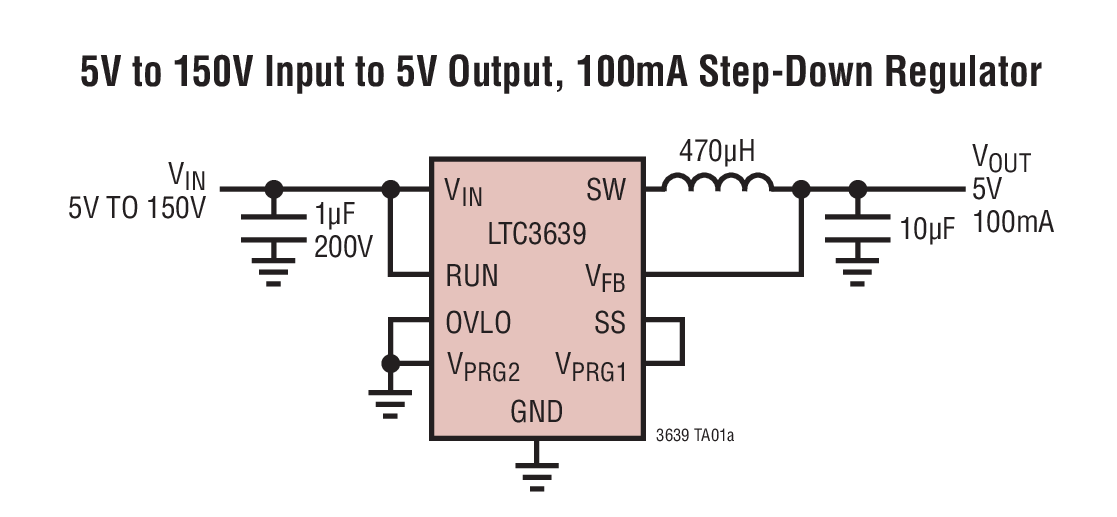
\includegraphics[width=0.8\linewidth]{document/Figure/LTC3639-1185.png}
    \caption{LTC3639-1185}
    \label{fig:LTC3639-1185}
\end{figure}
\newpage
\section{Task 1} \label{sec:Task1}

Die aufgebaute Schaltung mit dem LTC3639 und der zur Verfügung gestellten Eingangsschaltung gemäß Abbildung \ref{fig:LTC3639OhneFilter} wurde unter Berücksichtigung der Herstellerempfehlungen für die Beschaltung des LTC3639 umgesetzt. Alle externen Bauelemente, wie Induktivitäten, Kondensatoren und Widerstände, wurden entsprechend den Vorgaben des Herstellers gewählt, um eine optimale Leistung und Stabilität der Schaltung zu gewährleisten. Diese Auslegung stellt sicher, dass der LTC3639 unter den vorgesehenen Betriebsbedingungen effizient arbeitet.


\begin{figure}[H]
    \centering
    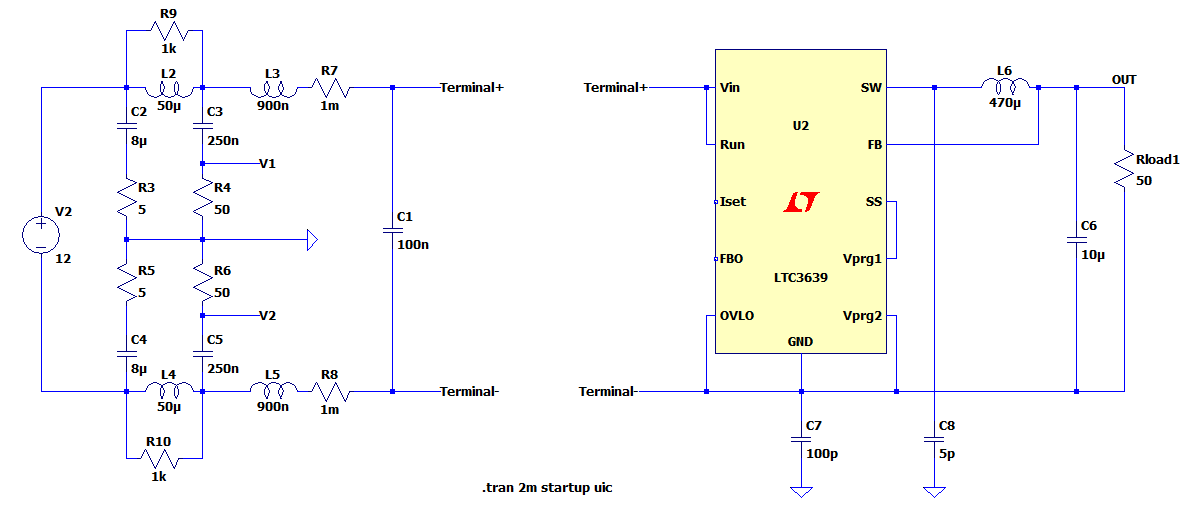
\includegraphics[width=0.8\linewidth]{document/Figure/LTC3639OhneFilter.png}
    \caption{LTC3639 ohne Filter}
    \label{fig:LTC3639OhneFilter}
\end{figure}

\subsection{FFT}

In Abbildung \ref{fig:LTC3639OhneFilterFFT} ist der FFT-Plot der Schaltung ohne Filter zu sehen. Hier zeigt sich, dass die Common-Mode- und Differential-Mode-Interferenzen deutlich über den zulässigen Grenzwerten für die EMV-Zertifizierung liegen. Ohne die Filterung treten hohe Störpegel auf, die die elektromagnetische Verträglichkeit der Schaltung negativ beeinflussen und eine Nicht-Zulassung für die EMV-Zertifizierung zur Folge haben würden.


\begin{figure}[H]
    \centering
    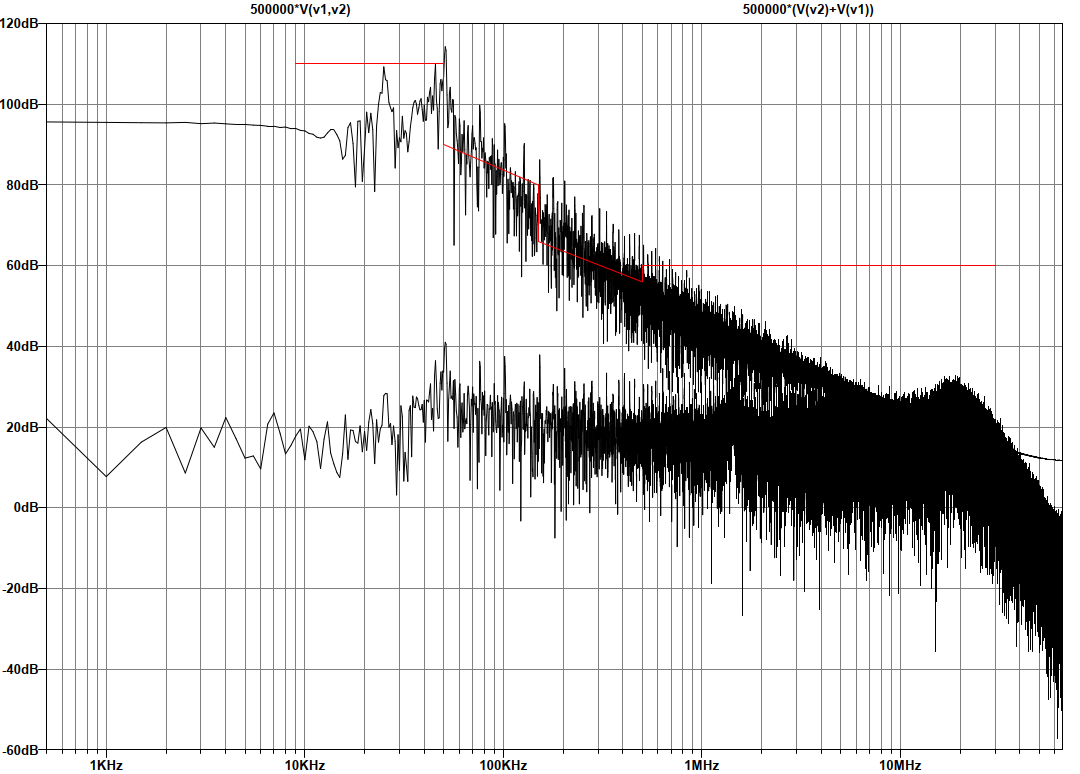
\includegraphics[width=0.8\linewidth]{document/Figure/LTC3639OhneFilterFFT.png}
    \caption{LTC3639 ohne Filter}
    \label{fig:LTC3639OhneFilterFFT}
\end{figure}



\newpage
\section{Task 2} \label{sec:Task2}

Für die Auslegung des Filters wurden die theoretischen Werte der benötigten Bauelemente berechnet, um die Cutoff-Frequenz optimal anzupassen und unerwünschte Störungen zu reduzieren. Ein Filterdesign, das in der Vorlesung besprochen wurde, wurde verwendet, um Resonanzspitzen zu unterdrücken. Eine zusätzliche Dämpfungsstruktur (Damping Branch) wurde integriert, um die Effektivität des Filters weiter zu steigern.

Die Schaltung in abbildung \ref{fig:LTC3639MitFilter} wurde um diesen Filter erweitert, um die EMV-Richtlinien einzuhalten und die leitungsgebundenen Emissionen sowohl im Common-Mode- als auch im Differential-Mode-Bereich zu reduzieren. Abbildung 2 zeigt die erweiterte Schaltung mit dem implementierten Filter, das zur Verbesserung der elektromagnetischen Verträglichkeit beiträgt.

Aufgaben und Auswahl der Komponenten:

\begin{itemize}
    \item \( C_f \) wirkt auf hohe Frequenzen und muss daher ein hochwertiger Kondensator sein, idealerweise ein Keramikkondensator.
    \item \( D_c \) beeinflusst niedrige Frequenzen und kann ein günstiger Elektrolytkondensator sein.
    \item \( C_d \) ist etwa 10- bis 20-mal größer als \( C_f \), um eine effektive Filterwirkung zu gewährleisten.
\end{itemize}

Dieses Design sorgt für eine effektive Dämpfung sowohl von differenziellen als auch von Gleichtaktstörungen und trägt dazu bei, die EMV-Anforderungen zu erfüllen. 

1. Induktivität \(L_f\):
\begin{equation}
    L_f = \frac{\left(\frac{1}{f_g \cdot 2 \pi}\right)^2}{C_f}
    \label{eqn:EffektiveKonvergenzordnung}
\end{equation} 

2. Charakteristischer Widerstand \(R_0\):
\begin{equation}
    R_0 = \sqrt{\frac{L_f}{C_f}}
    \label{eqn:EffektiveKonvergenzordnung}
\end{equation} 

3. Modifizierte Kapazität \(C_d\):
\begin{equation}
    C_d = C_{\text{faktor}} \cdot C_f
    \label{eqn:EffektiveKonvergenzordnung}
\end{equation} 

4. Verhältnis \(n\):
\begin{equation}
    n = \frac{C_d}{C_f}
    \label{eqn:EffektiveKonvergenzordnung}
\end{equation} 

5. Dämpfungswiderstand \(R_d\):
\begin{equation}
    R_d = R_0 \cdot \sqrt{\frac{(2 + n)(4 + 3n)}{(2n)^2(4 + n)}}
    \label{eqn:EffektiveKonvergenzordnung}
\end{equation} 


\begin{figure}[H]
    \centering
    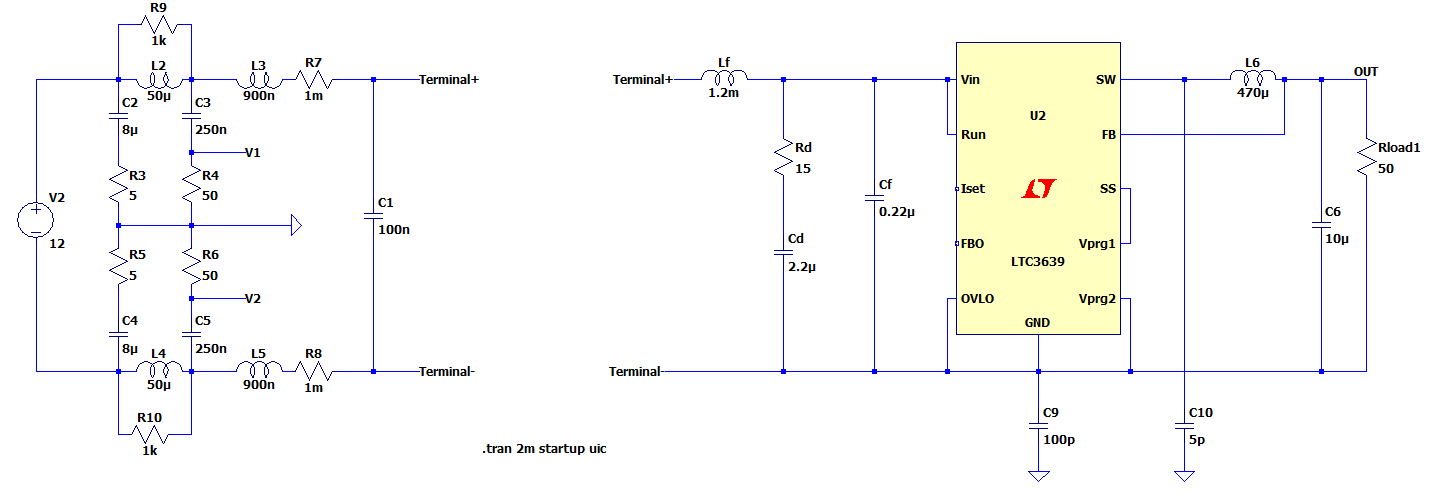
\includegraphics[width=0.8\linewidth]{document/Figure/LTC3639MitFilter.png}
    \caption{LTC3639 mit Filter}
    \label{fig:LTC3639MitFilter}
\end{figure}


\subsection{FFT}

In Abbildung \ref{fig:LTC3639MitFilterFFT} ist der FFT-Plot der Schaltung mit integriertem Filter dargestellt. Es ist erkennbar, dass der Filter seine Funktion erfüllt, indem er sowohl die Common-Mode- als auch die Differential-Mode-Störungen wirksam reduziert und unter die zulässigen Grenzwerte für die EMV-Zertifizierung verschiebt.


\begin{figure}[H]
    \centering
    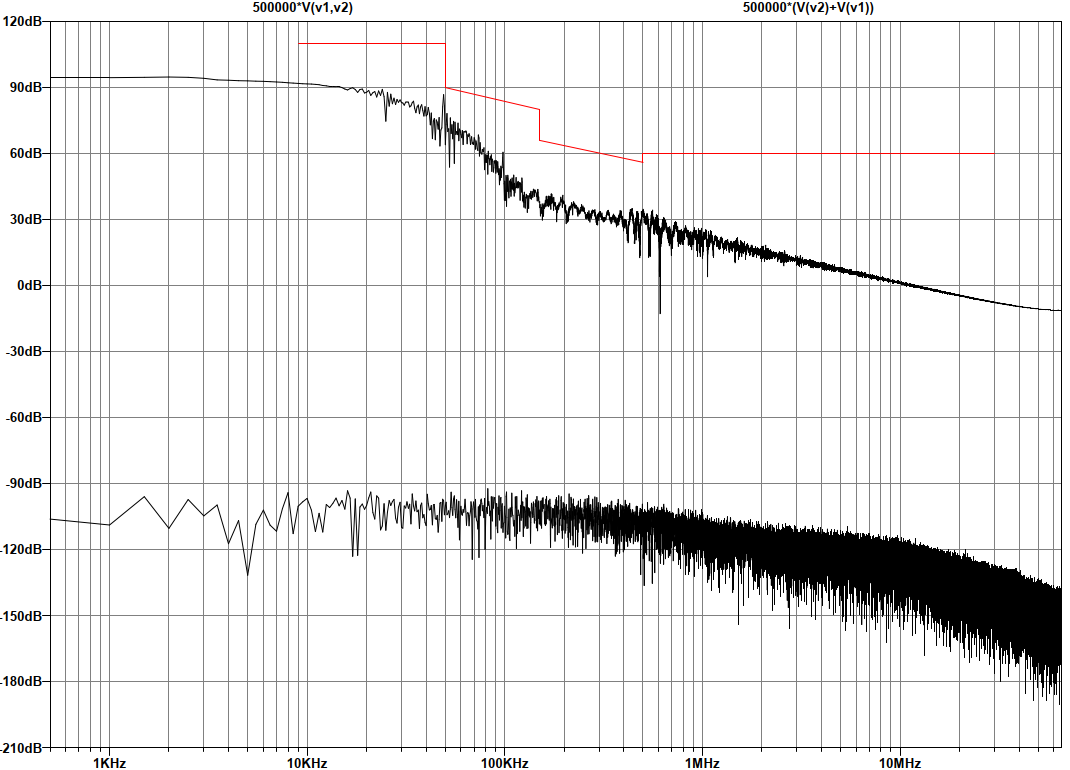
\includegraphics[width=0.8\linewidth]{document/Figure/LTC3639MitFilterFFT.png}
    \caption{FFT LTC3639 mit Filter}
    \label{fig:LTC3639MitFilterFFT}
\end{figure}
\newpage
\section{Layout-Empfehlungen für das Board-Design}\label{sec:Layout}

Für ein EMV-konformes Design mit dem LTC3639 sollten folgende Punkte beachtet werden:

\begin{enumerate}
    \item \textbf{Kondensatoren nahe den Pins des LTC3639} platzieren, um parasitäre Induktivitäten und Widerstände zu minimieren.
    \item \textbf{Masseverbindungen} durch ein durchgehendes Masse-Plane sicherstellen, um Rauschen und Spannungsdifferenzen zu reduzieren.
    \item \textbf{Schleifenflächen minimieren}, um elektromagnetische Störungen zu verringern.
    \item \textbf{Hochfrequenz- und Niedrigfrequenzkomponenten} räumlich oder auf verschiedenen Plane-Ebenen trennen.
    \item \textbf{Thermisches Management} durch ausreichende Kühlflächen für Wärmequellen wie den LTC3639.
    \item \textbf{Filterkomponenten} nah an den Regleranschlüssen platzieren, um leitungsgebundene Störungen zu dämpfen.
    \item \textbf{Signalpfade kurz halten} und unnötige Kreuzungen zwischen Hoch- und Niedrigfrequenzleitungen vermeiden.
    \item \textbf{Stromversorgungsleitungen} breit und direkt führen, um Spannungsabfälle und Erwärmung zu minimieren.
\end{enumerate}

Diese Maßnahmen verbessern die EMV-Leistung und die Zuverlässigkeit des Designs.


\newpage
% =============================================================================

\clearpage

%% -> Verzeichnisse
\pagestyle{fancy}
\pagenumbering{Roman}
\addtocounter{romanPagenumber}{1}
\setcounter{page}{\theromanPagenumber}
%% --------------------------------------------------------------------- %%
\clearpage
%Appendix
\clearpage
\fancyhead[L]{}
\fancyhead[R]{\MakeUppercase{ANHANG}}
\appendix 
\addcontentsline{toc}{section}{ANHANG}
\section{Anhang}\label{app:1} 

\end{document}

% Verzeichnisse
% alles was danach kommt in römischer Seitennummerierung
\clearpage
\pagenumbering{Roman}
\setcounter{page}{\value{RoemischeSeiten}}
% gilt für alle Verzeichnisse
\fancyhead[R]{\sffamily\bfseries\MakeUppercase{\headerLists}}

% Abbildungsverzeichnis
\fancyhead[L]{\listfigurename}
\fancyhead[R]{}
\phantomsection
\addcontentsline{toc}{section}{\listfigurename}
\listoffigures

%Tabellenverzeichnis
\clearpage
\phantomsection
\fancyhead[L]{\listtablename}
\addcontentsline{toc}{section}{\listtablename}
\listoftables

%Quellcodeverzeichnis
%\clearpage
%\phantomsection
%\fancyhead[L]{\lstlistlistingname}
%\addcontentsline{toc}{section}{\lstlistlistingname}
%\lstlistoflistings

%Literaturverzeichnis
\clearpage
\bibliographystyle{IEEEtran}
\fancyhead[L]{\refname}
\phantomsection
\addcontentsline{toc}{section}{\refname}
\bibliography{literatur}

%Appendix
\clearpage
\fancyhead[L]{}
\fancyhead[R]{\MakeUppercase{\appendixname}}
\appendix 
\addcontentsline{toc}{section}{\appendixname}
%========================PREPARATION===================================
\section{Preparation} \label{appendix:preparation}

\subsection{First preparation} \label{appendix:firstpreparation}
\FloatBarrier
\begin{figure}[ht]
    \begin{center}
    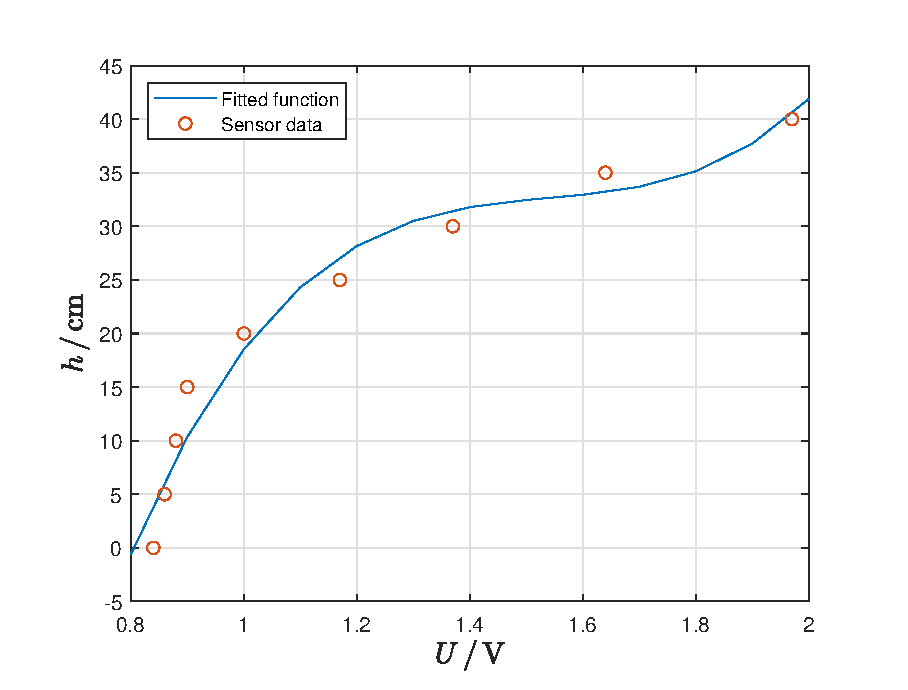
\includegraphics[angle=0,width=0.6\textwidth]{figure/fittedFunction.eps}
    \end{center}
    \caption[Fitted function for first lab preparation]
    {Fitted function $h(u) = (73.36 \cdot u^3) + (-339.13 \cdot u^2) + (527.23 \cdot u) + (-242.94)$}
    \label{fig:fittedFunction}
\end{figure}
\FloatBarrier

\subsection{Second preparation} \label{appendix:secondpreparation}
\FloatBarrier
\begin{figure}[ht]
	\begin{center}
        % trim = left bottom right top
		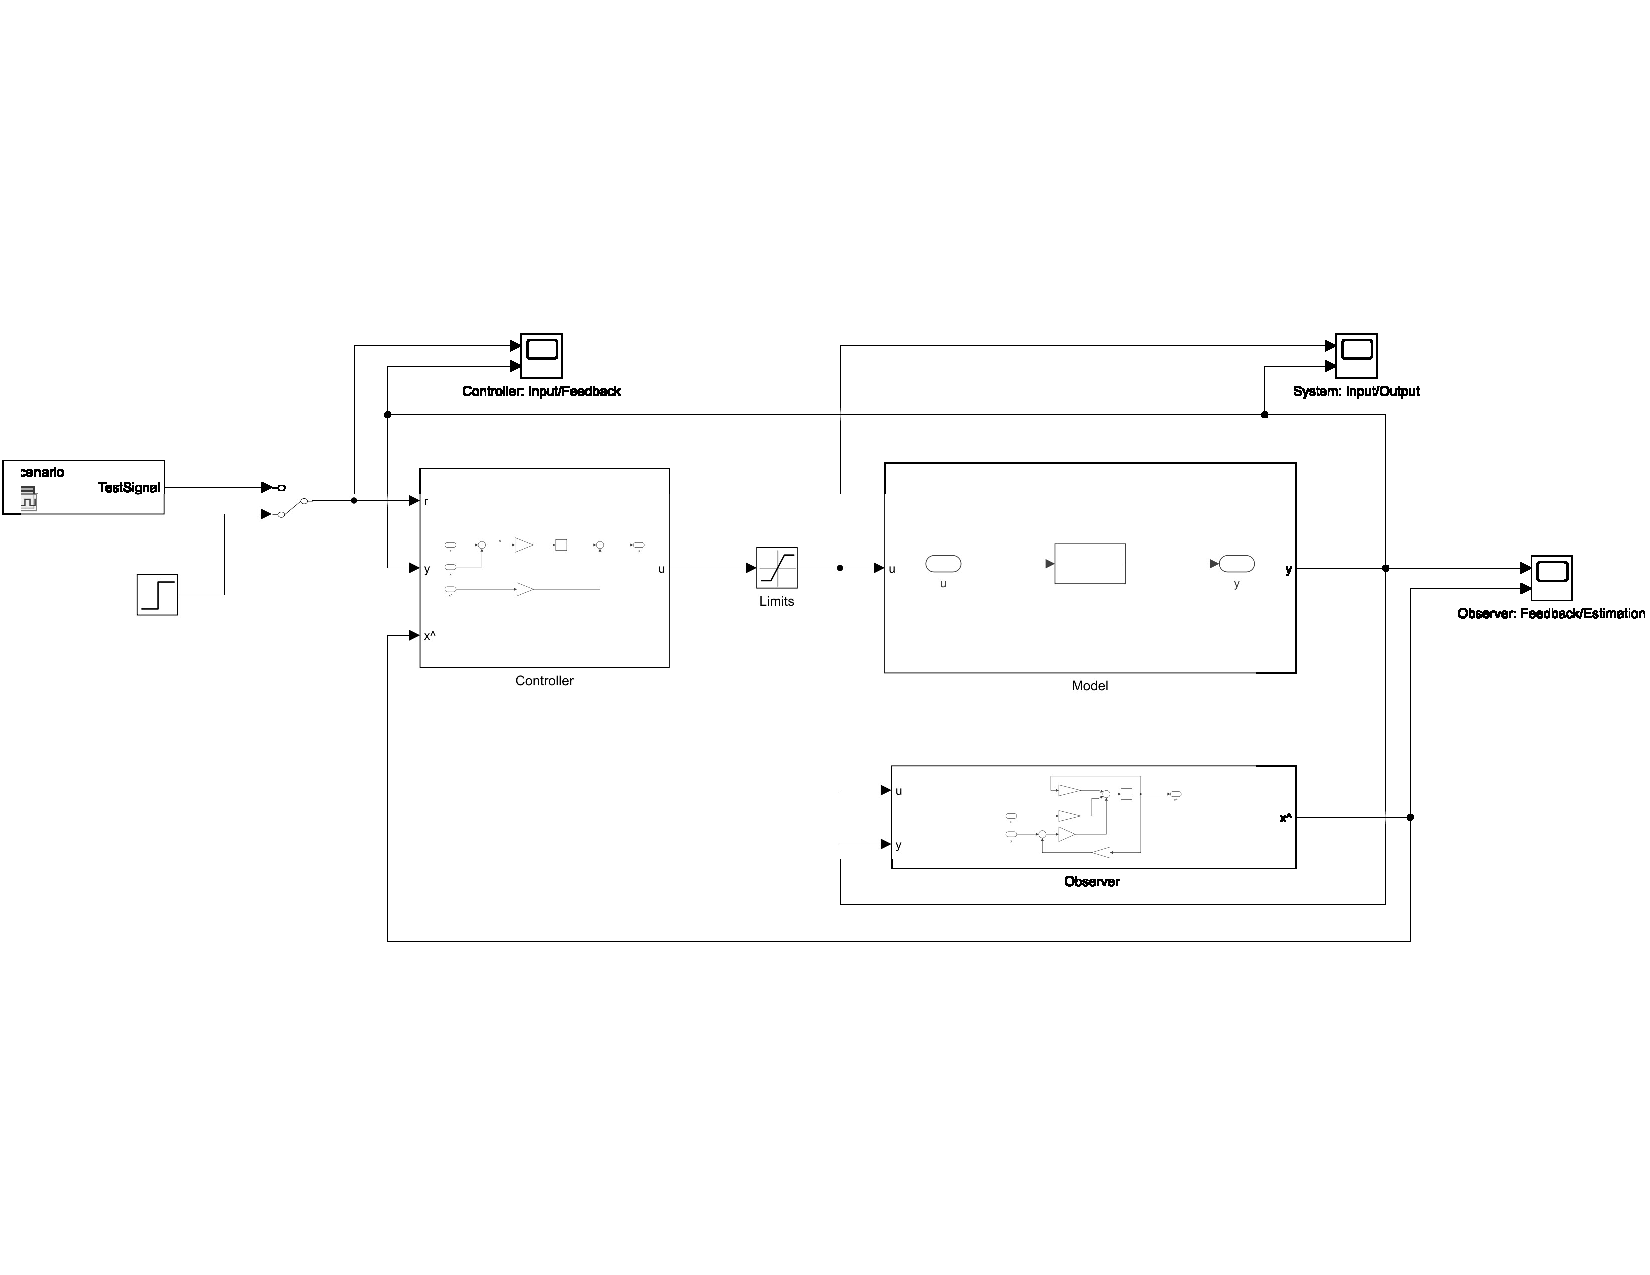
\includegraphics[clip, trim=0cm 5cm 0cm 5cm, width=1\textwidth]{simulink/simulinkSimulation.pdf}
		\caption[Simulink simulation of the control system]{Simulink simulation of the control system}
		\label{fig:simuSimulation}
	\end{center}
\end{figure}
\FloatBarrier

\FloatBarrier
\begin{figure}[ht]
	\begin{center}
        % trim = left bottom right top
		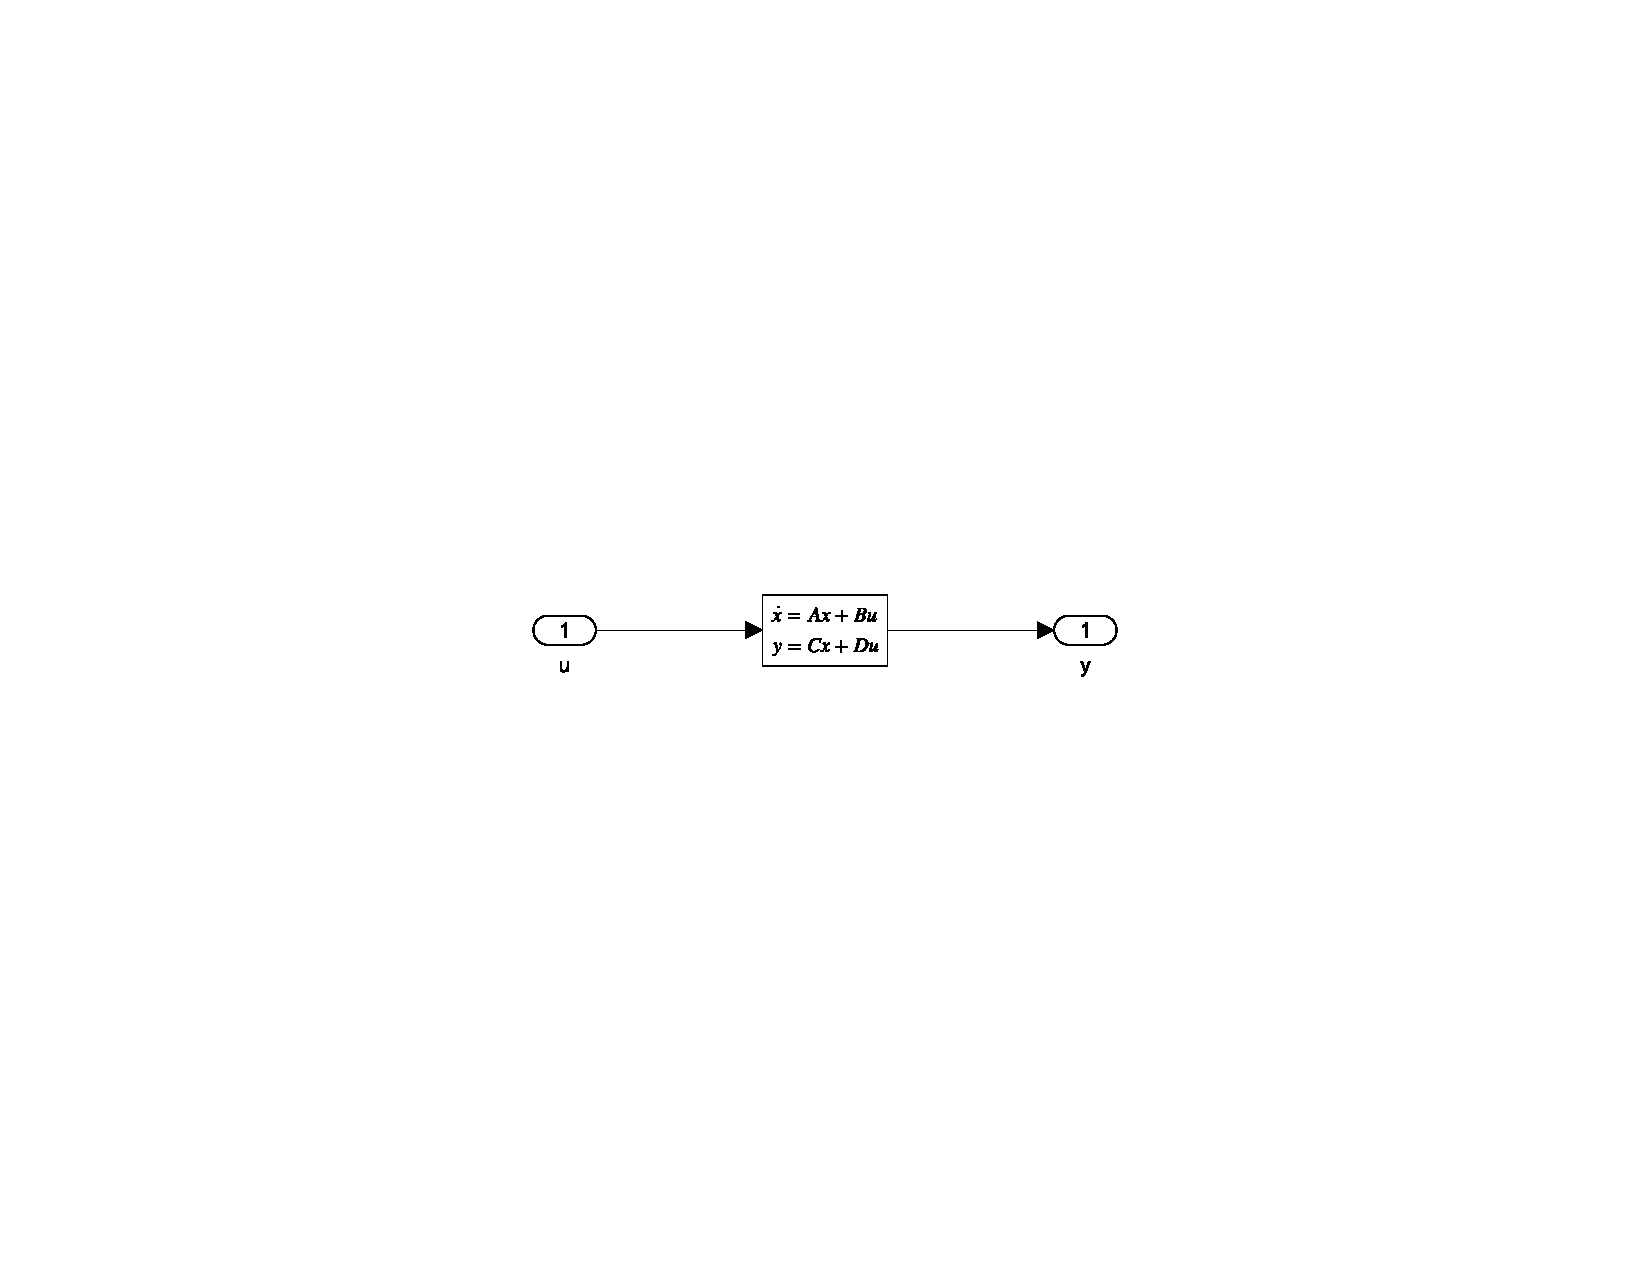
\includegraphics[clip, trim=0cm 10cm 0cm 8cm, width=1\textwidth]{simulink/simulinkModel.pdf}
		\caption[Simulink model of the system]{Simulink model of the system}
		\label{fig:simuModel}
	\end{center}
\end{figure}
\FloatBarrier

\FloatBarrier
\begin{figure}[ht]
	\begin{center}
        % trim = left bottom right top
		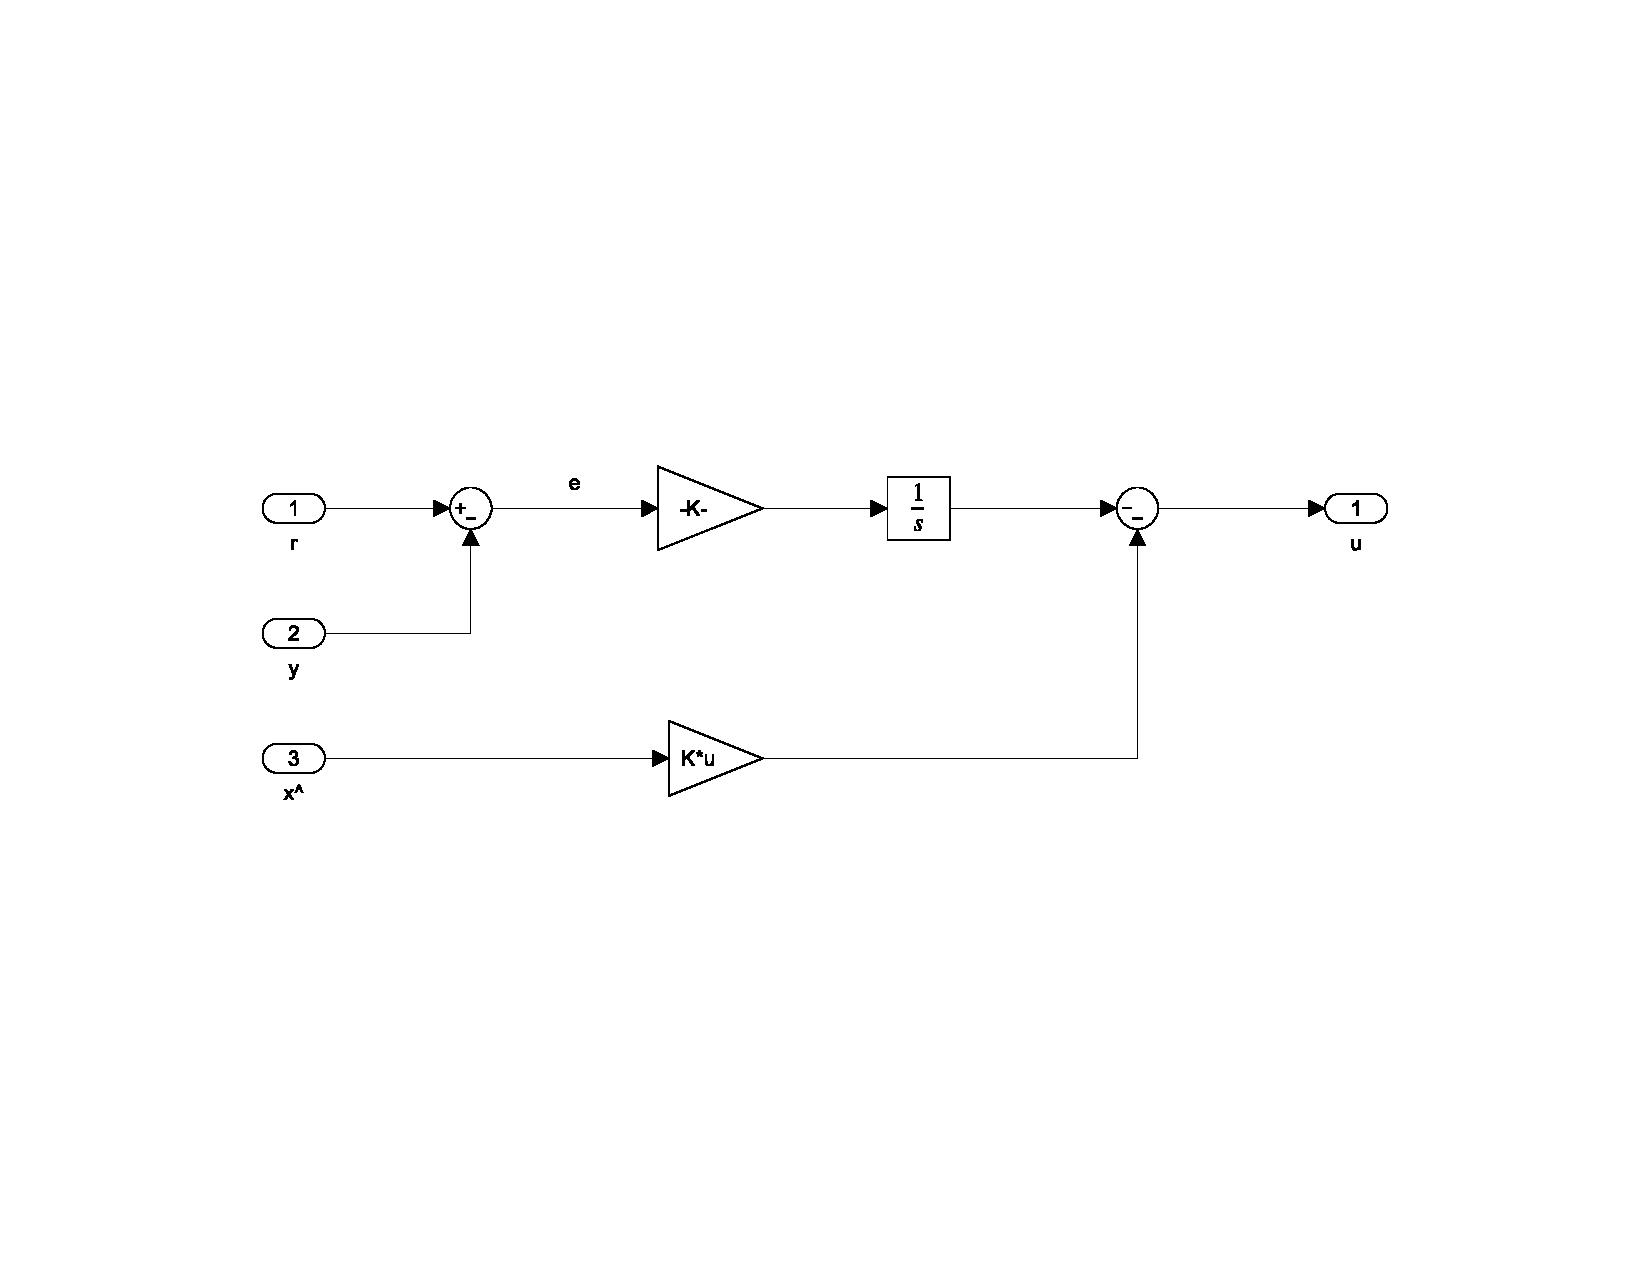
\includegraphics[clip, trim=0cm 8cm 0cm 8cm, width=1\textwidth]{simulink/simulinkController.pdf}
		\caption[Simulink controller]{Simulink controller}
		\label{fig:simuController}
	\end{center}
\end{figure}
\FloatBarrier

\FloatBarrier
\begin{figure}[ht]
	\begin{center}
        % trim = left bottom right top
		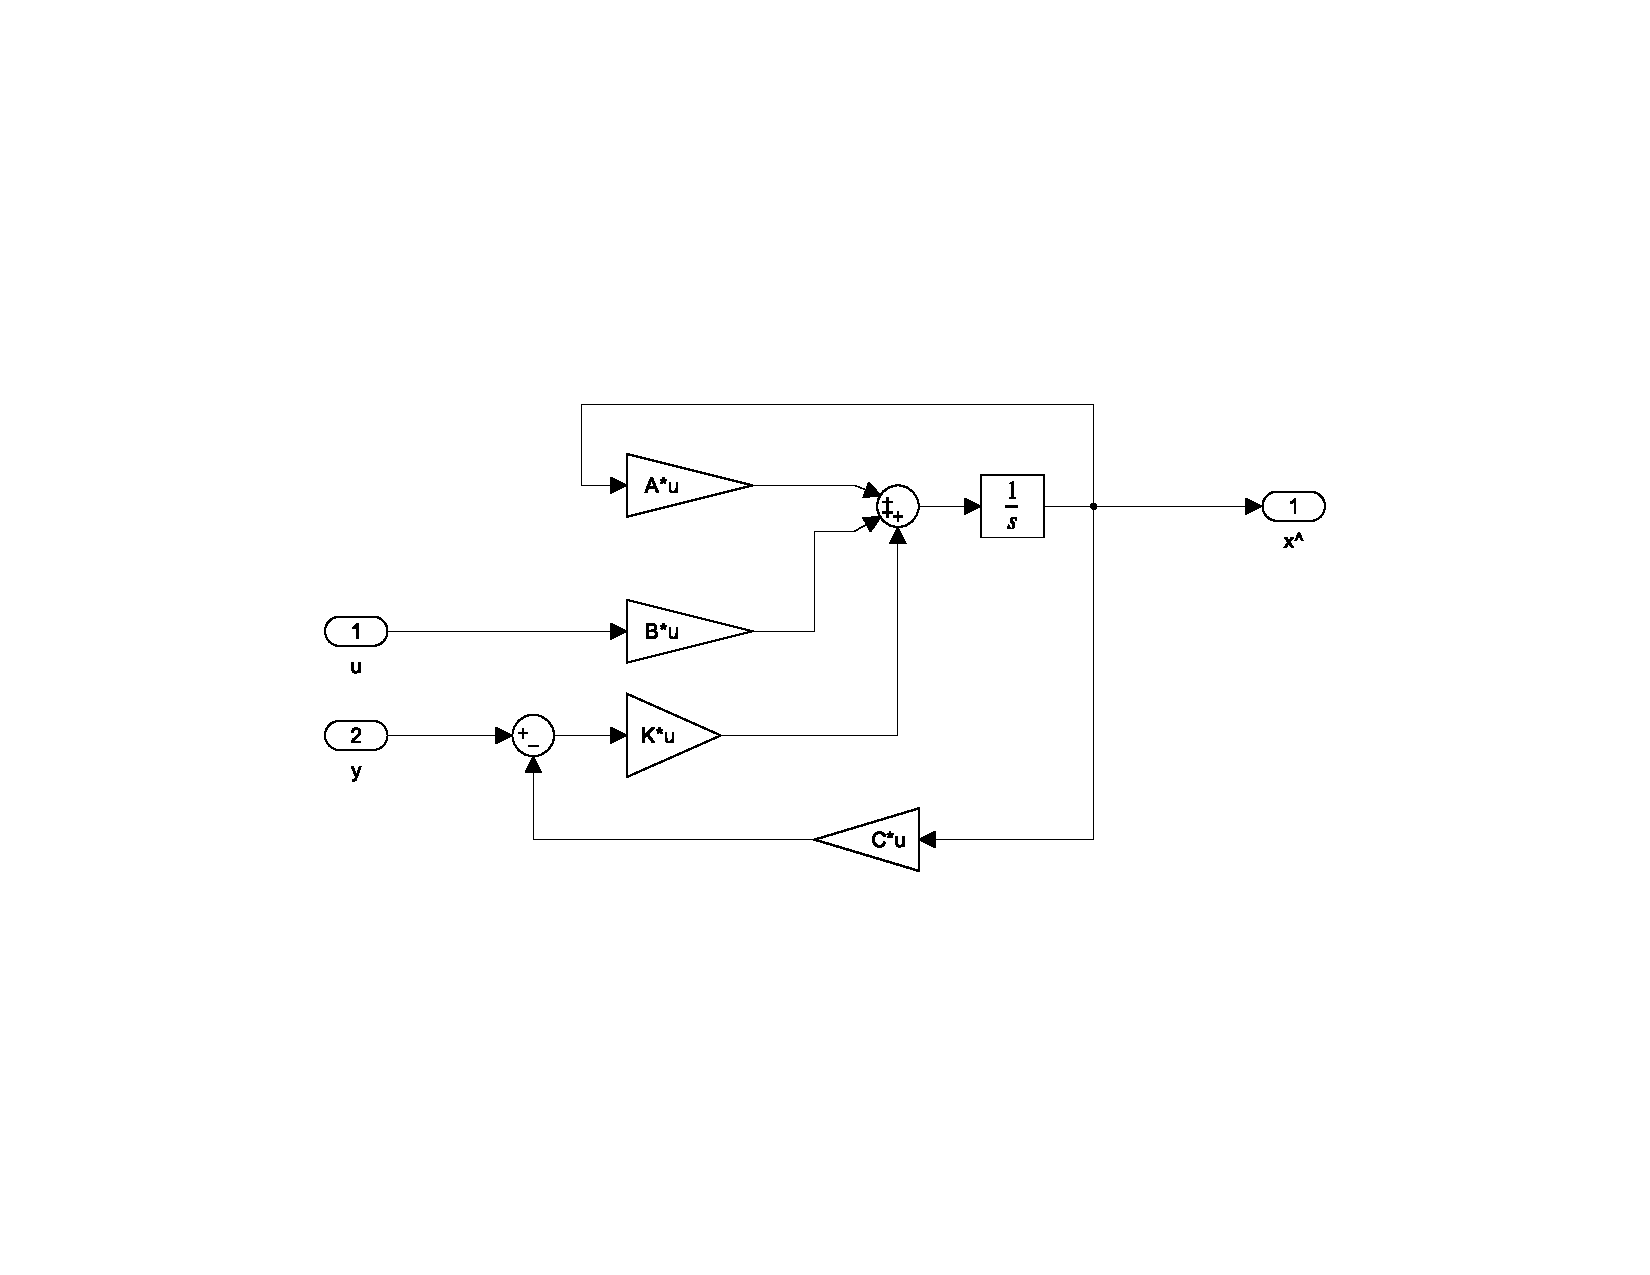
\includegraphics[clip, trim=0cm 6.5cm 0cm 6cm, width=1\textwidth]{simulink/simulinkObserver.pdf}
		\caption[Simulink observer]{Simulink observer}
		\label{fig:simuObserver}
	\end{center}
\end{figure}
\FloatBarrier

\FloatBarrier
\begin{figure}[ht]
    \centering
    \begin{subfigure}[b]{0.45\textwidth}
    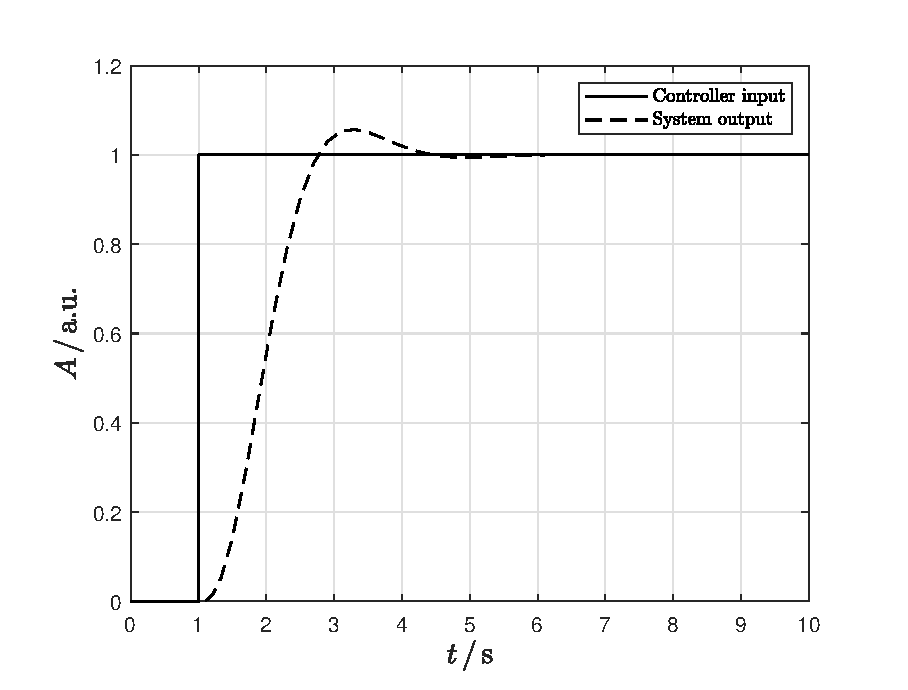
\includegraphics[width=\textwidth]{simulink/simulinkPlotStepController.eps}
    \caption{}
    \label{subfig:stepController}
    \end{subfigure}
    \begin{subfigure}[b]{0.45\textwidth}
    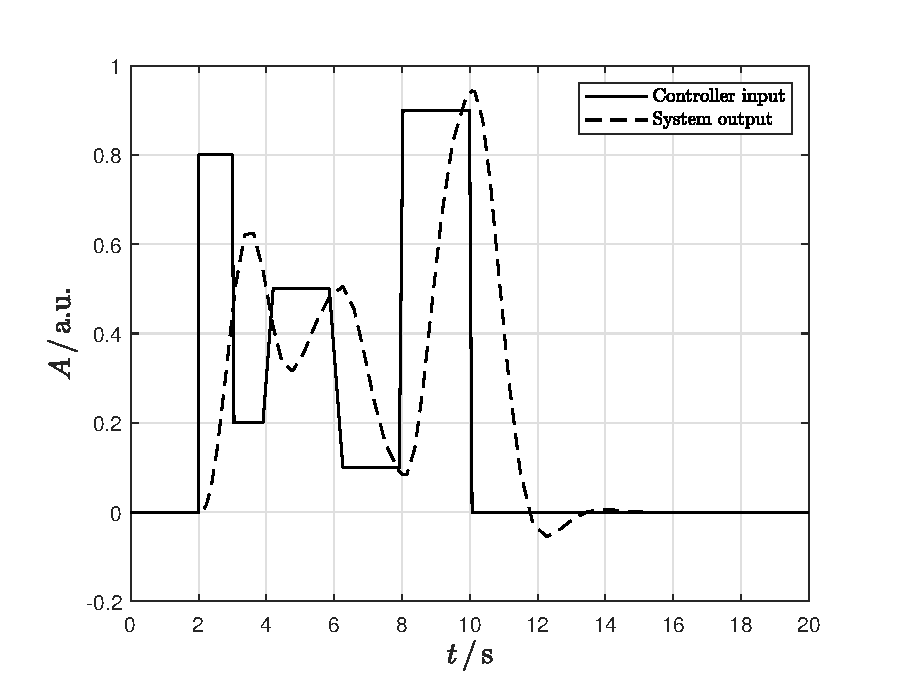
\includegraphics[width=\textwidth]{simulink/simulinkPlotTrajectoryController.eps}
    \caption{}
    \label{subfig:trajController}
    \end{subfigure}

    \hfill
    
    \begin{subfigure}[b]{0.45\textwidth}
    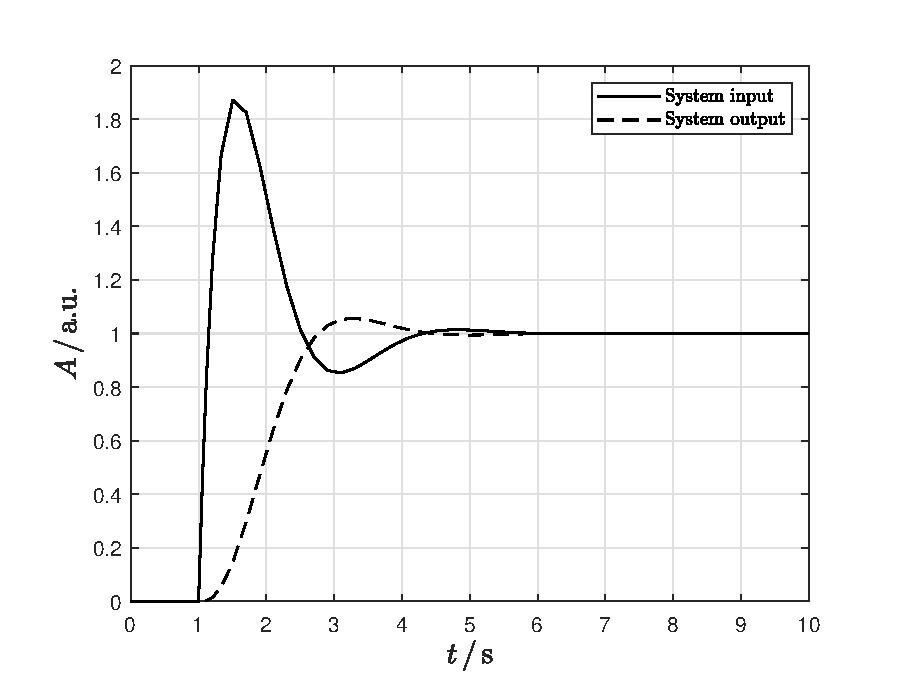
\includegraphics[width=\textwidth]{simulink/simulinkPlotStepSystem.eps}
    \caption{}
    \label{subfig:stepSystem}
    \end{subfigure}
    \begin{subfigure}[b]{0.45\textwidth}
    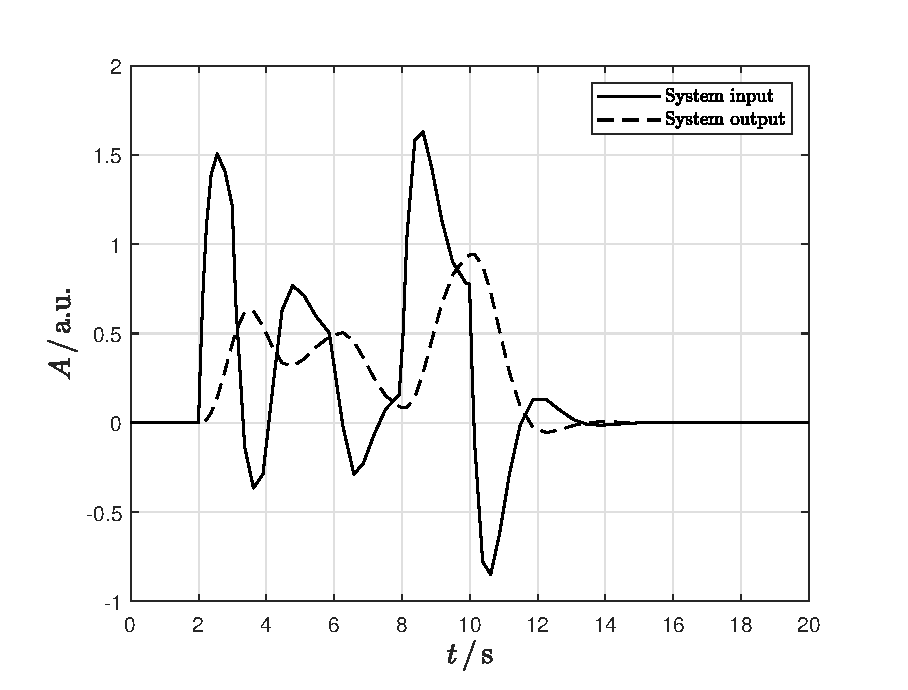
\includegraphics[width=\textwidth]{simulink/simulinkPlotTrajectorySystem.eps}
    \caption{}
    \label{subfig:trajSystem}
    \end{subfigure}

    \hfill
    
    \begin{subfigure}[b]{0.45\textwidth}
    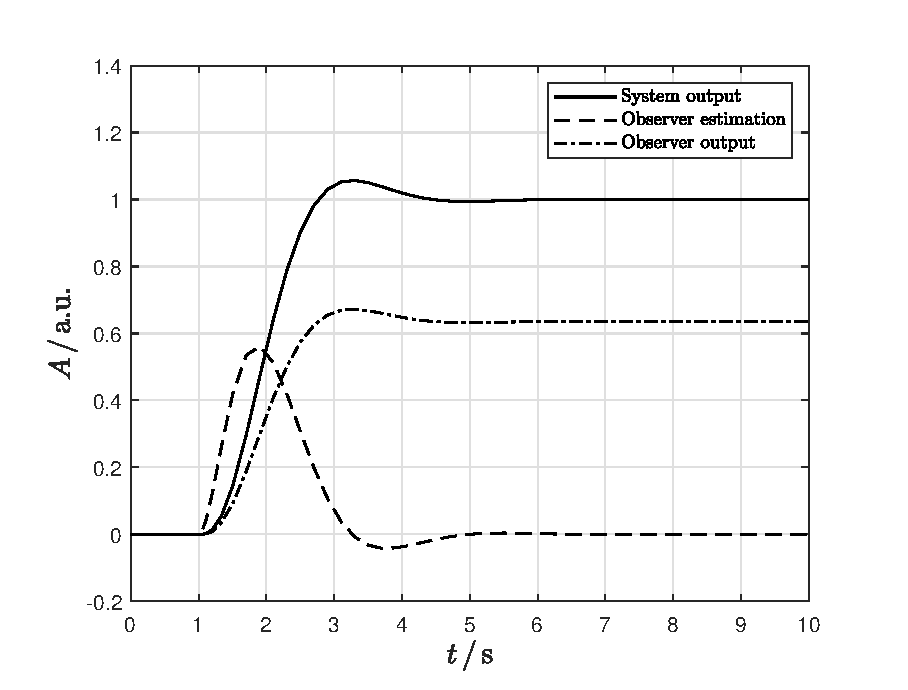
\includegraphics[width=\textwidth]{simulink/simulinkPlotStepObserver.eps}
    \caption{}
    \label{subfig:stepObserver}
    \end{subfigure}
    \begin{subfigure}[b]{0.45\textwidth}
    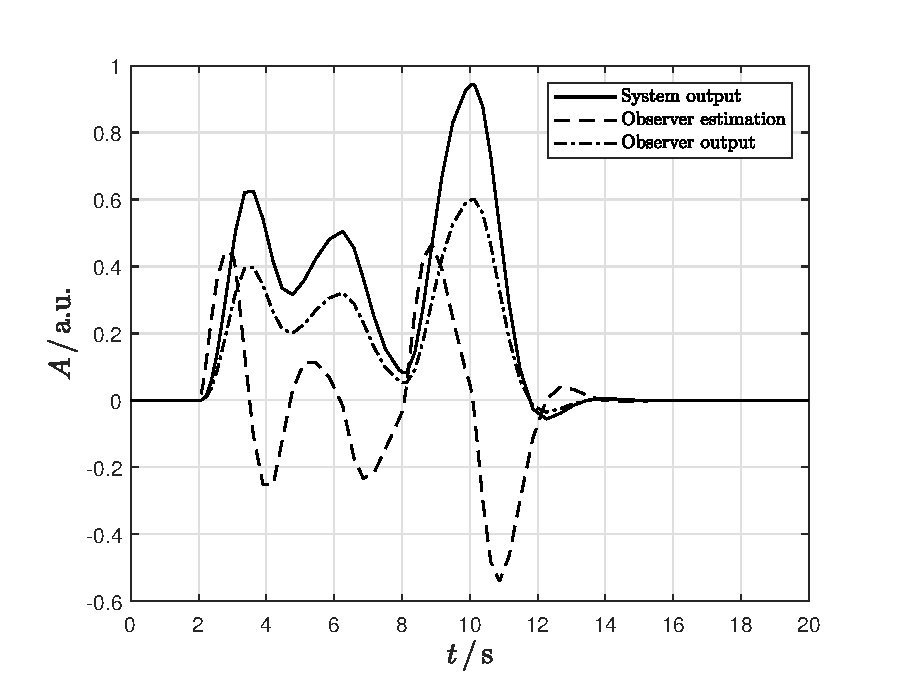
\includegraphics[width=\textwidth]{simulink/simulinkPlotTrajectoryObserver.eps}
    \caption{}
    \label{subfig:trajObserver}
    \end{subfigure}

    \hfill
    
    \caption[Simulations in Simulink]{Left for step input with (a) controller (c) system and (e) observer. Right trajectory input with (b) controller (d) system and (f) observer.}
    \label{fig:simulations}
\end{figure}
\FloatBarrier


\newpage


%========================DATA===================================
\section{Laboratory} \label{appendix:data}

\subsection{Sensor data} \label{appendix:sensordata}
\begin{table}[H]
\caption[Sensor output voltage against distance]{Sensor output voltage against distance} \label{tab:sensor}
\begin{center}
\begin{tabular}{ c c }
\toprule
Distance & Sensor voltage \\
\midrule\\
18  & 1.93 \\
23  & 1.91 \\
28  & 1.68 \\
33  & 1.32 \\
38  & 1.11 \\
43  & 0.96 \\
48  & 0.90 \\
53  & 0.88 \\
58  & 0.82 \\
\bottomrule
\end{tabular} 
\end{center}
\end{table} 

\FloatBarrier
\begin{figure}[ht]
    \begin{center}
    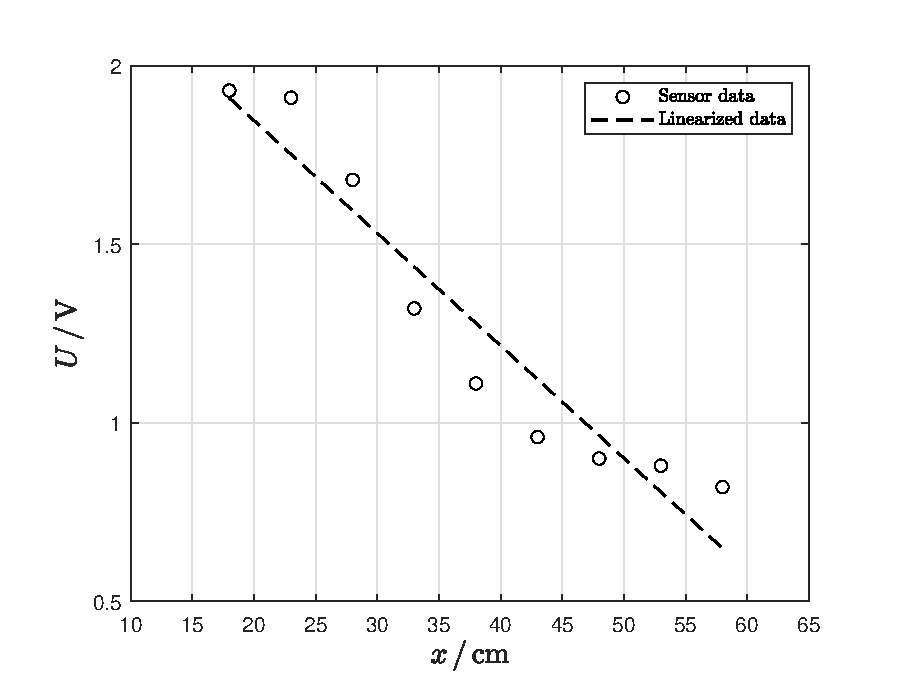
\includegraphics[angle=0,width=0.6\textwidth]{figure/sensorLinearized.eps}
    \end{center}
    \caption[Sensor linearization]
    {Sensor linearization: $f(x) = -0.0315*x + 2.4758888$}
    \label{fig:sensorLinearization}
\end{figure}
\FloatBarrier

\newpage

\subsection{System identification} \label{appendix:systemidentification}
\FloatBarrier
\begin{figure}[ht]
    \centering
    \begin{subfigure}[b]{0.45\textwidth}
    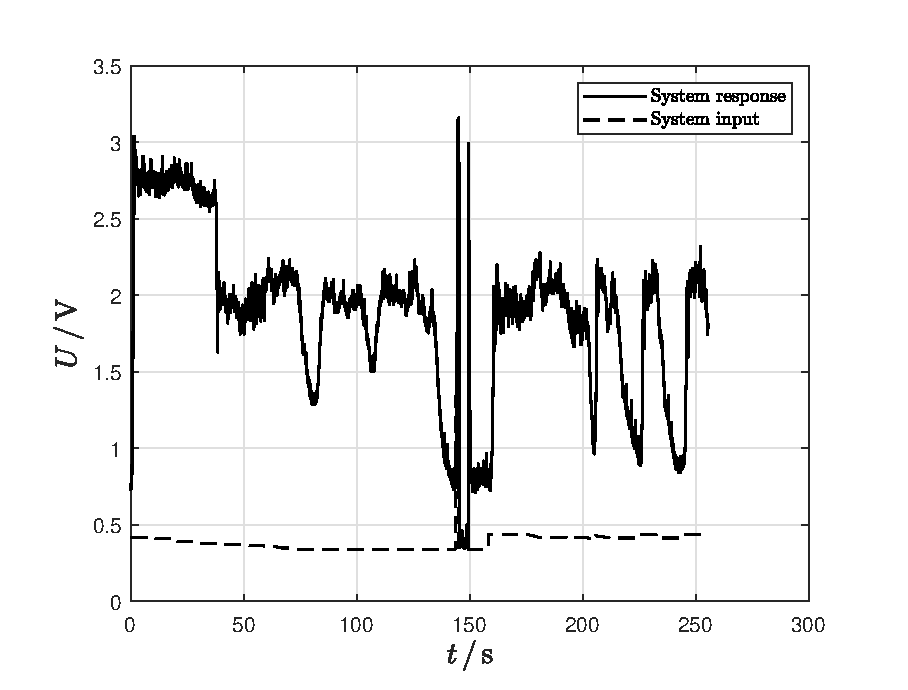
\includegraphics[width=\textwidth]{figure/raw.eps}
    \caption{}
    \label{subfig:raw}
    \end{subfigure}
    \begin{subfigure}[b]{0.45\textwidth}
    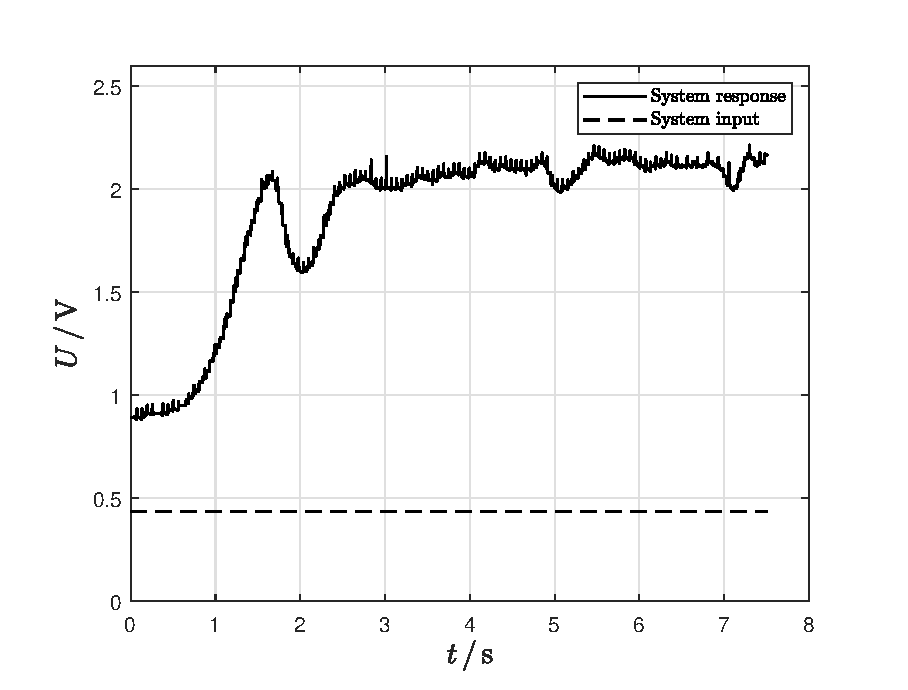
\includegraphics[width=\textwidth]{figure/trimming.eps}
    \caption{}
    \label{subfig:trimming}
    \end{subfigure}

    \hfill
    
    \begin{subfigure}[b]{0.45\textwidth}
    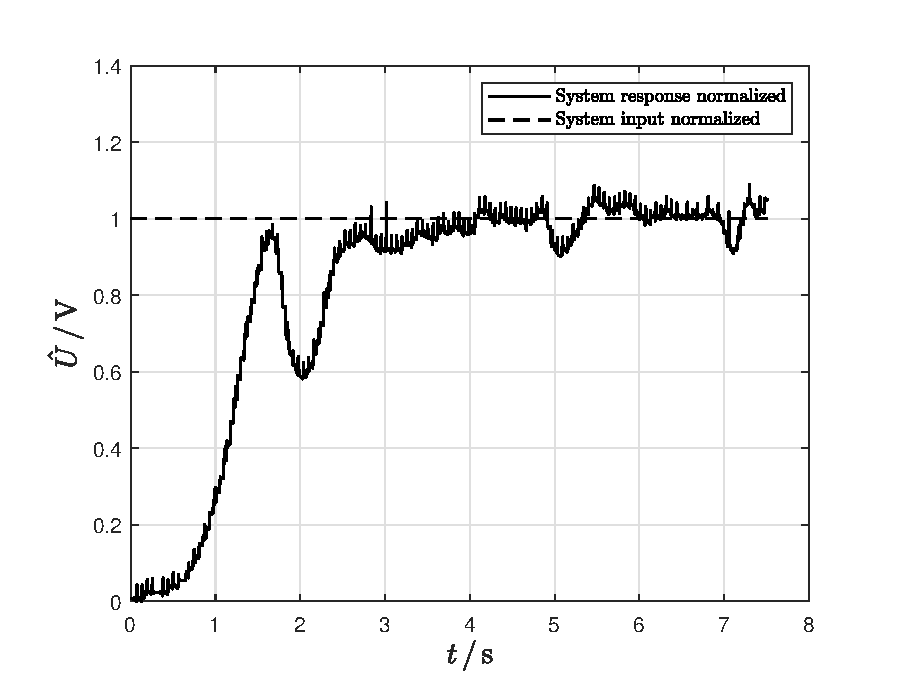
\includegraphics[width=\textwidth]{figure/normalize.eps}
    \caption{}
    \label{subfig:normalize}
    \end{subfigure}
    \begin{subfigure}[b]{0.45\textwidth}
    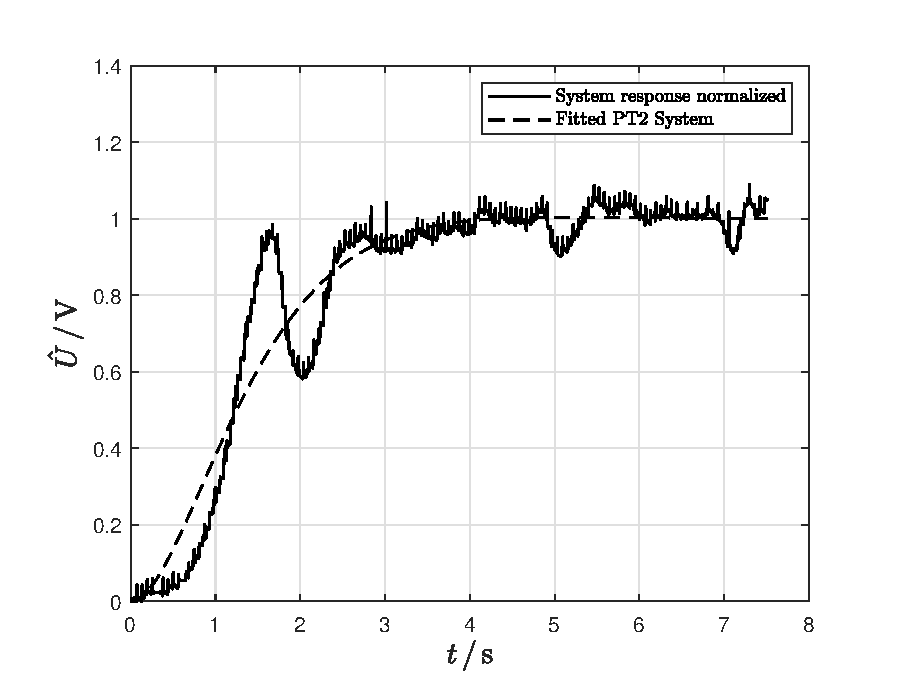
\includegraphics[width=\textwidth]{figure/fitting.eps}
    \caption{}
    \label{subfig:fitting}
    \end{subfigure}

    \hfill
    
    \caption[System identification in the laboratory]{(a) Raw data (b) Trimmed (c) Normalized (d) Fitted PT2 system}
\end{figure}
\FloatBarrier

\newpage

\subsection{Controller performance} \label{appendix:performance}
\FloatBarrier
\begin{figure}[ht]
	\begin{center}
        % trim = left bottom right top
		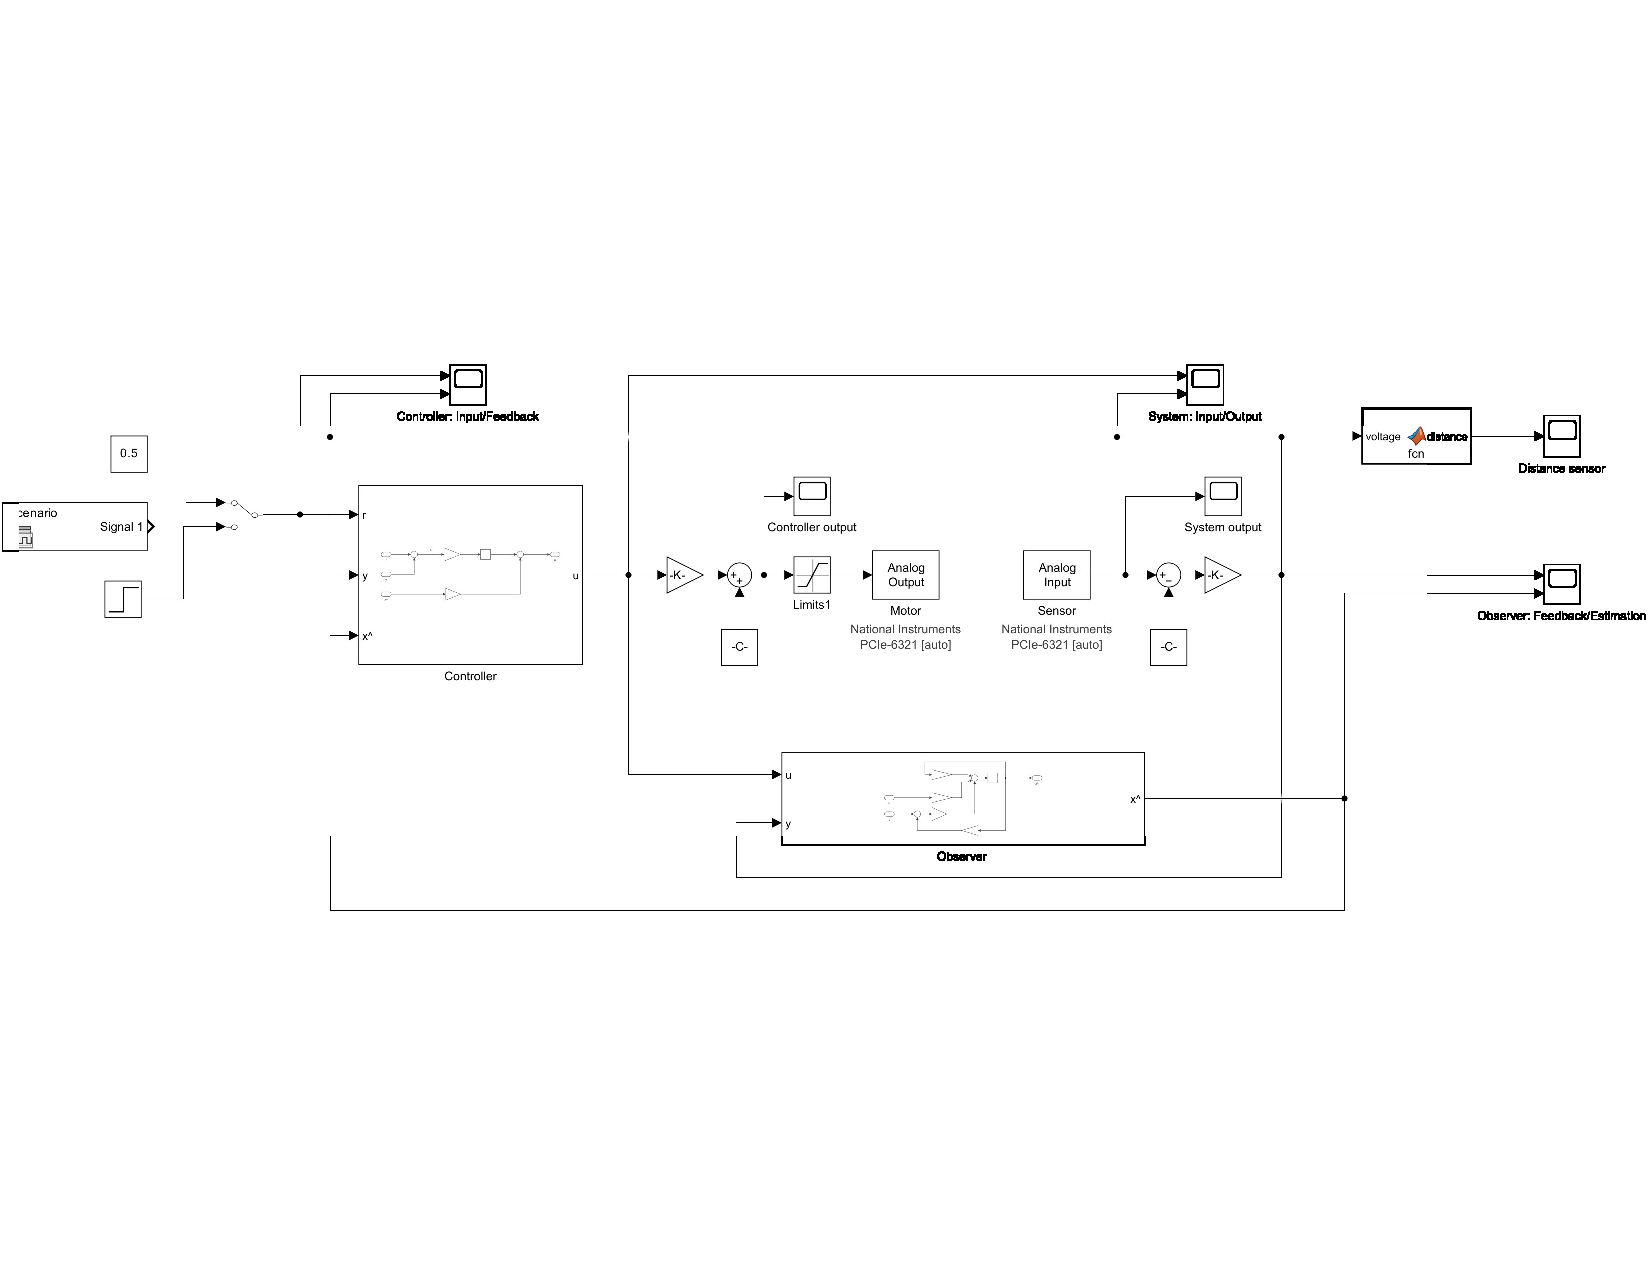
\includegraphics[clip, trim=0cm 6cm 0cm 6cm, width=0.8\textwidth]{simulink/simulinkLaboratory.pdf}
		\caption[Simulink laboratory application]{Simulink laboratory application}
		\label{fig:simuLaboratory}
	\end{center}
\end{figure}
\FloatBarrier

\FloatBarrier
\begin{figure}[ht]
    \begin{center}
    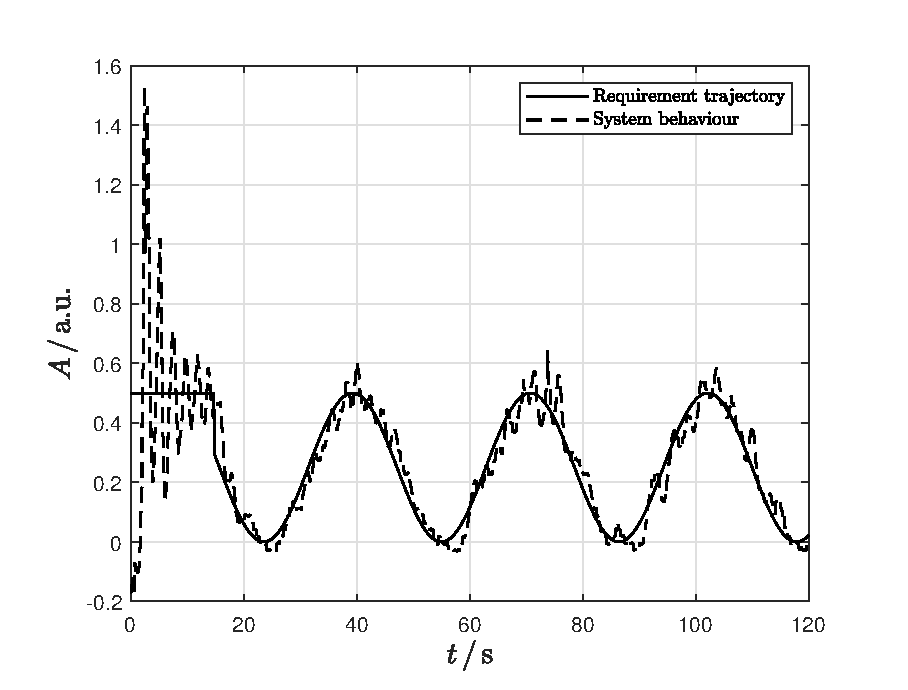
\includegraphics[angle=0,width=0.6\textwidth]{simulink/simulinkPlotTrajectoryLaboratory.eps}
    \end{center}
    \caption[System behaviour with sine wave trajectory]
    {System behaviour with sine wave trajectory}
    \label{fig:simuSineTrajectory}
\end{figure}
\FloatBarrier


\newpage


%========================MATLAB===================================
\section{MATLAB} \label{appendix:matlab}

\subsection{First laboratory}
\lstinputlisting[style=MStyle]{m_files/laboratory.m}
\subsubsection{Plots}
\lstinputlisting[style=MStyle]{m_files/plots.m}
\subsubsection{PT2 fitting function}
\lstinputlisting[style=MStyle]{m_files/unit_step_PT2.m}

\newpage

\subsection{Second laboratory}
\lstinputlisting[style=MStyle]{m_files/laboratory1.m} 

% letzte Fußzeile (MCI Logo)
\pagestyle{fancy}
\lfoot{
\includegraphics[height=0.9cm]{Images/MCIFuss.png}}
\newpage
\lfoot{}

\end{document}